\section{Results}

I decided to simulate polynomials up to $\mathbf{10^{th}}$ degree.

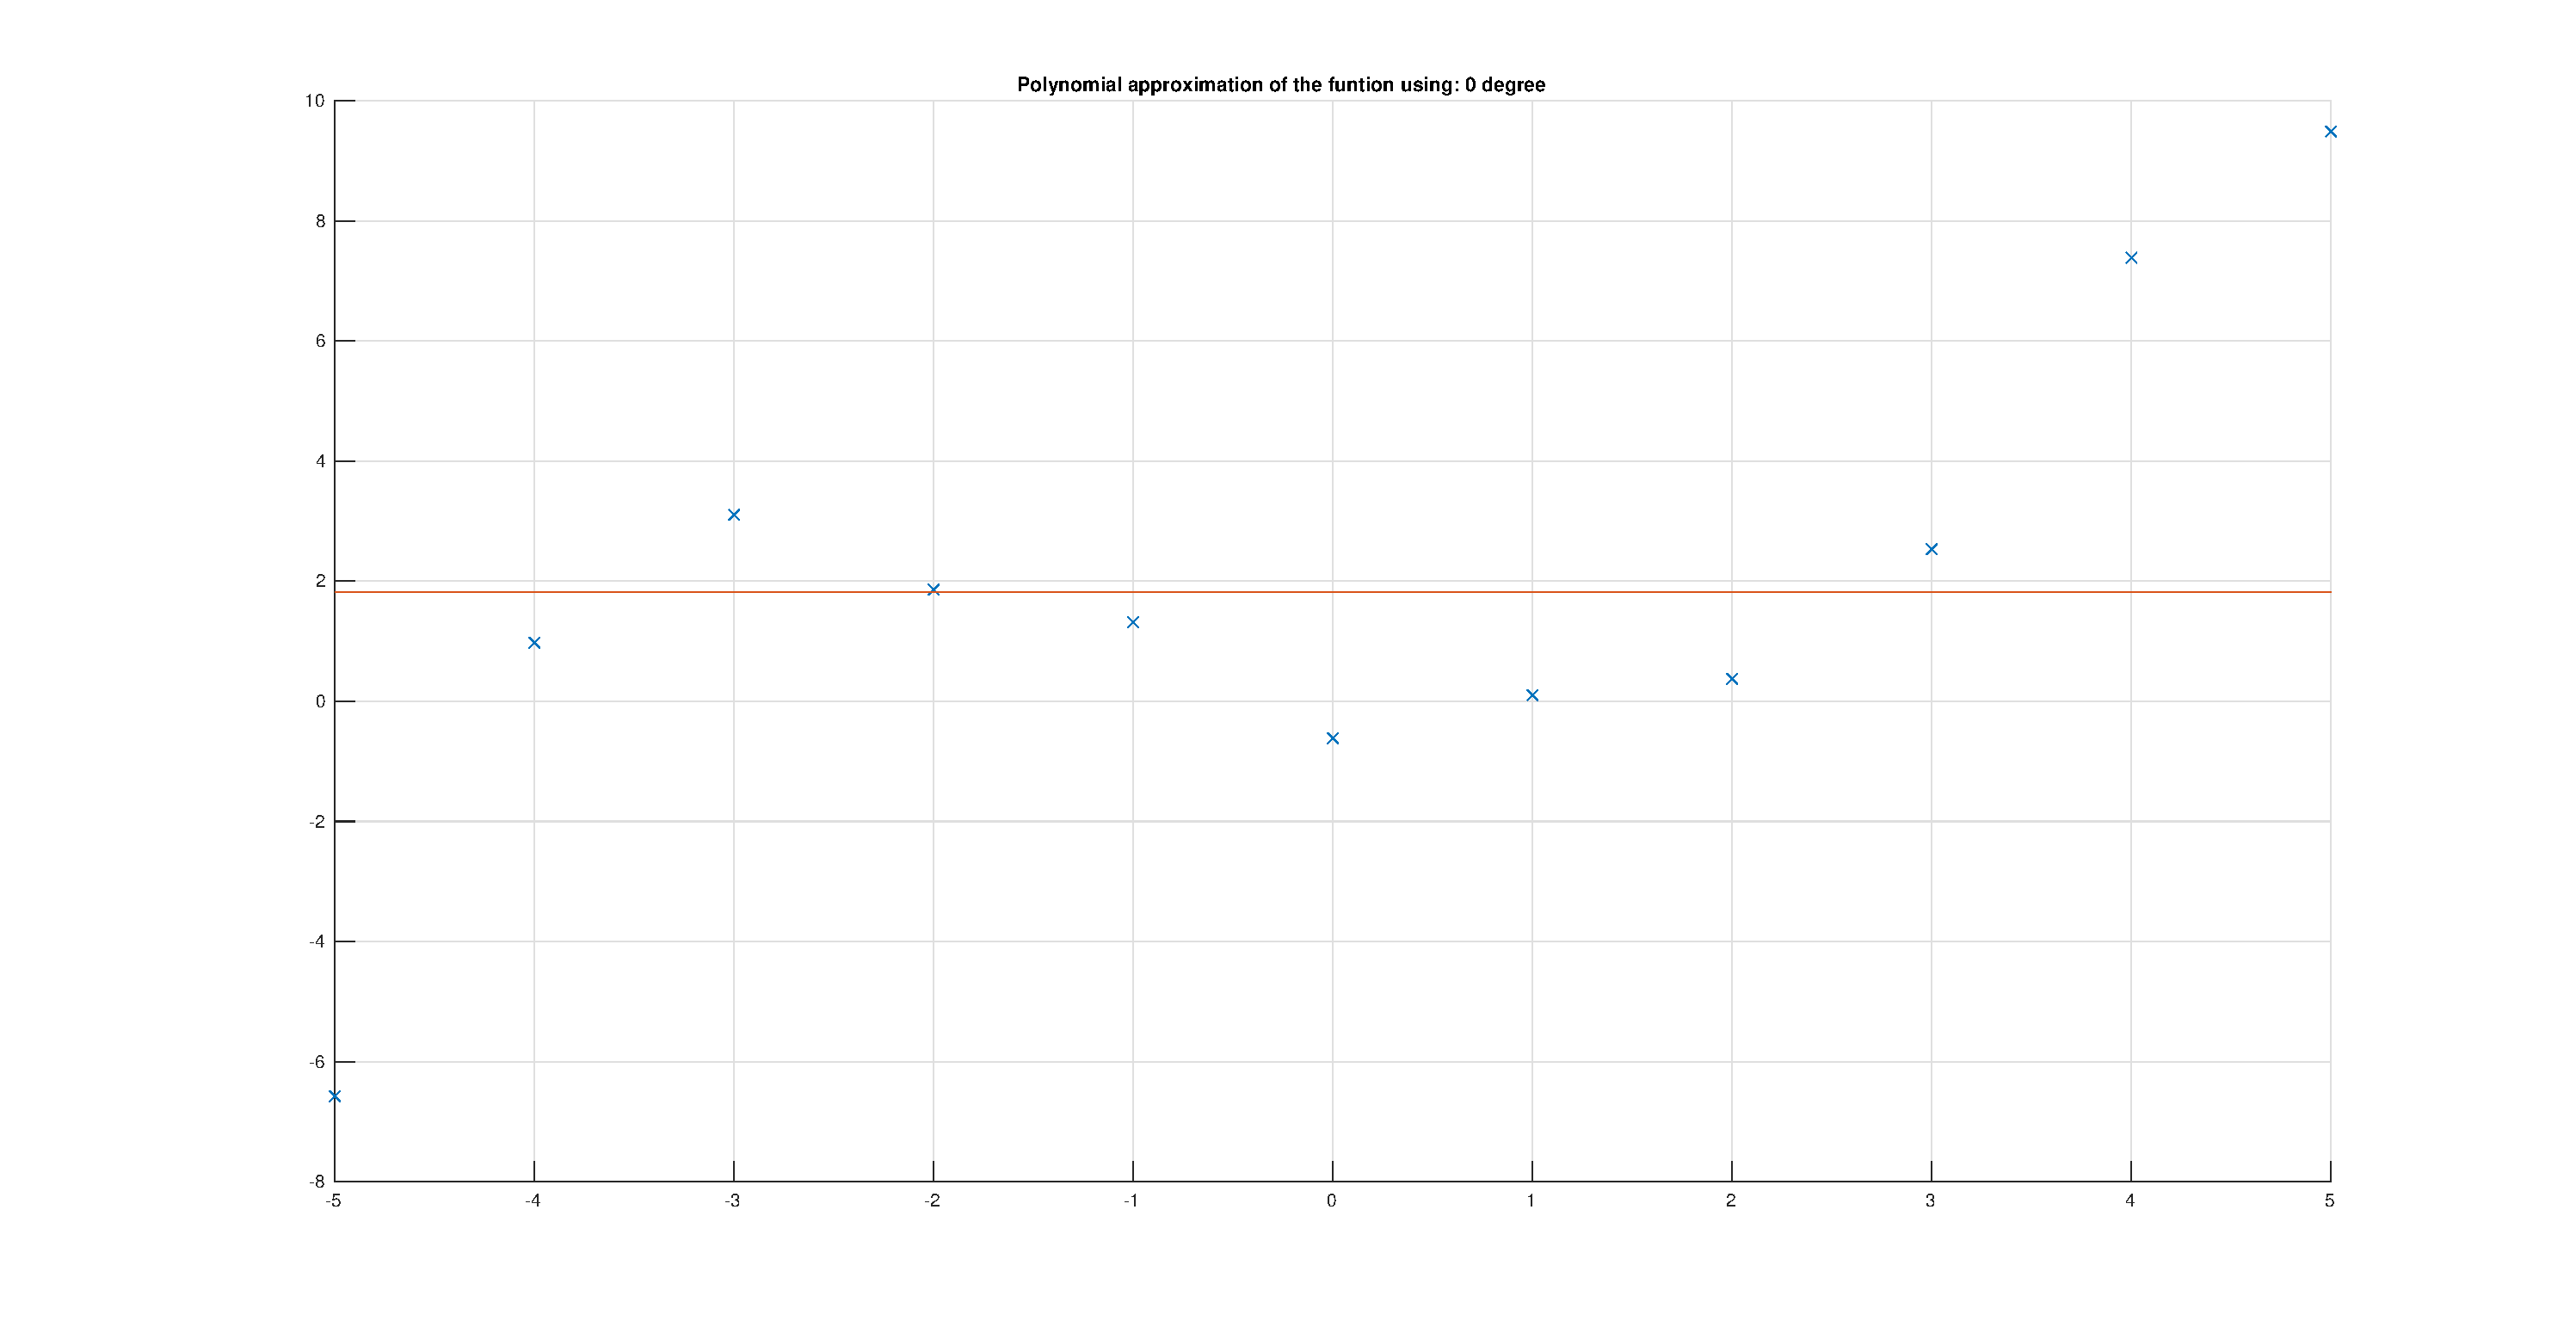
\includepdf[pages=-]{10-eps-converted-to.pdf}
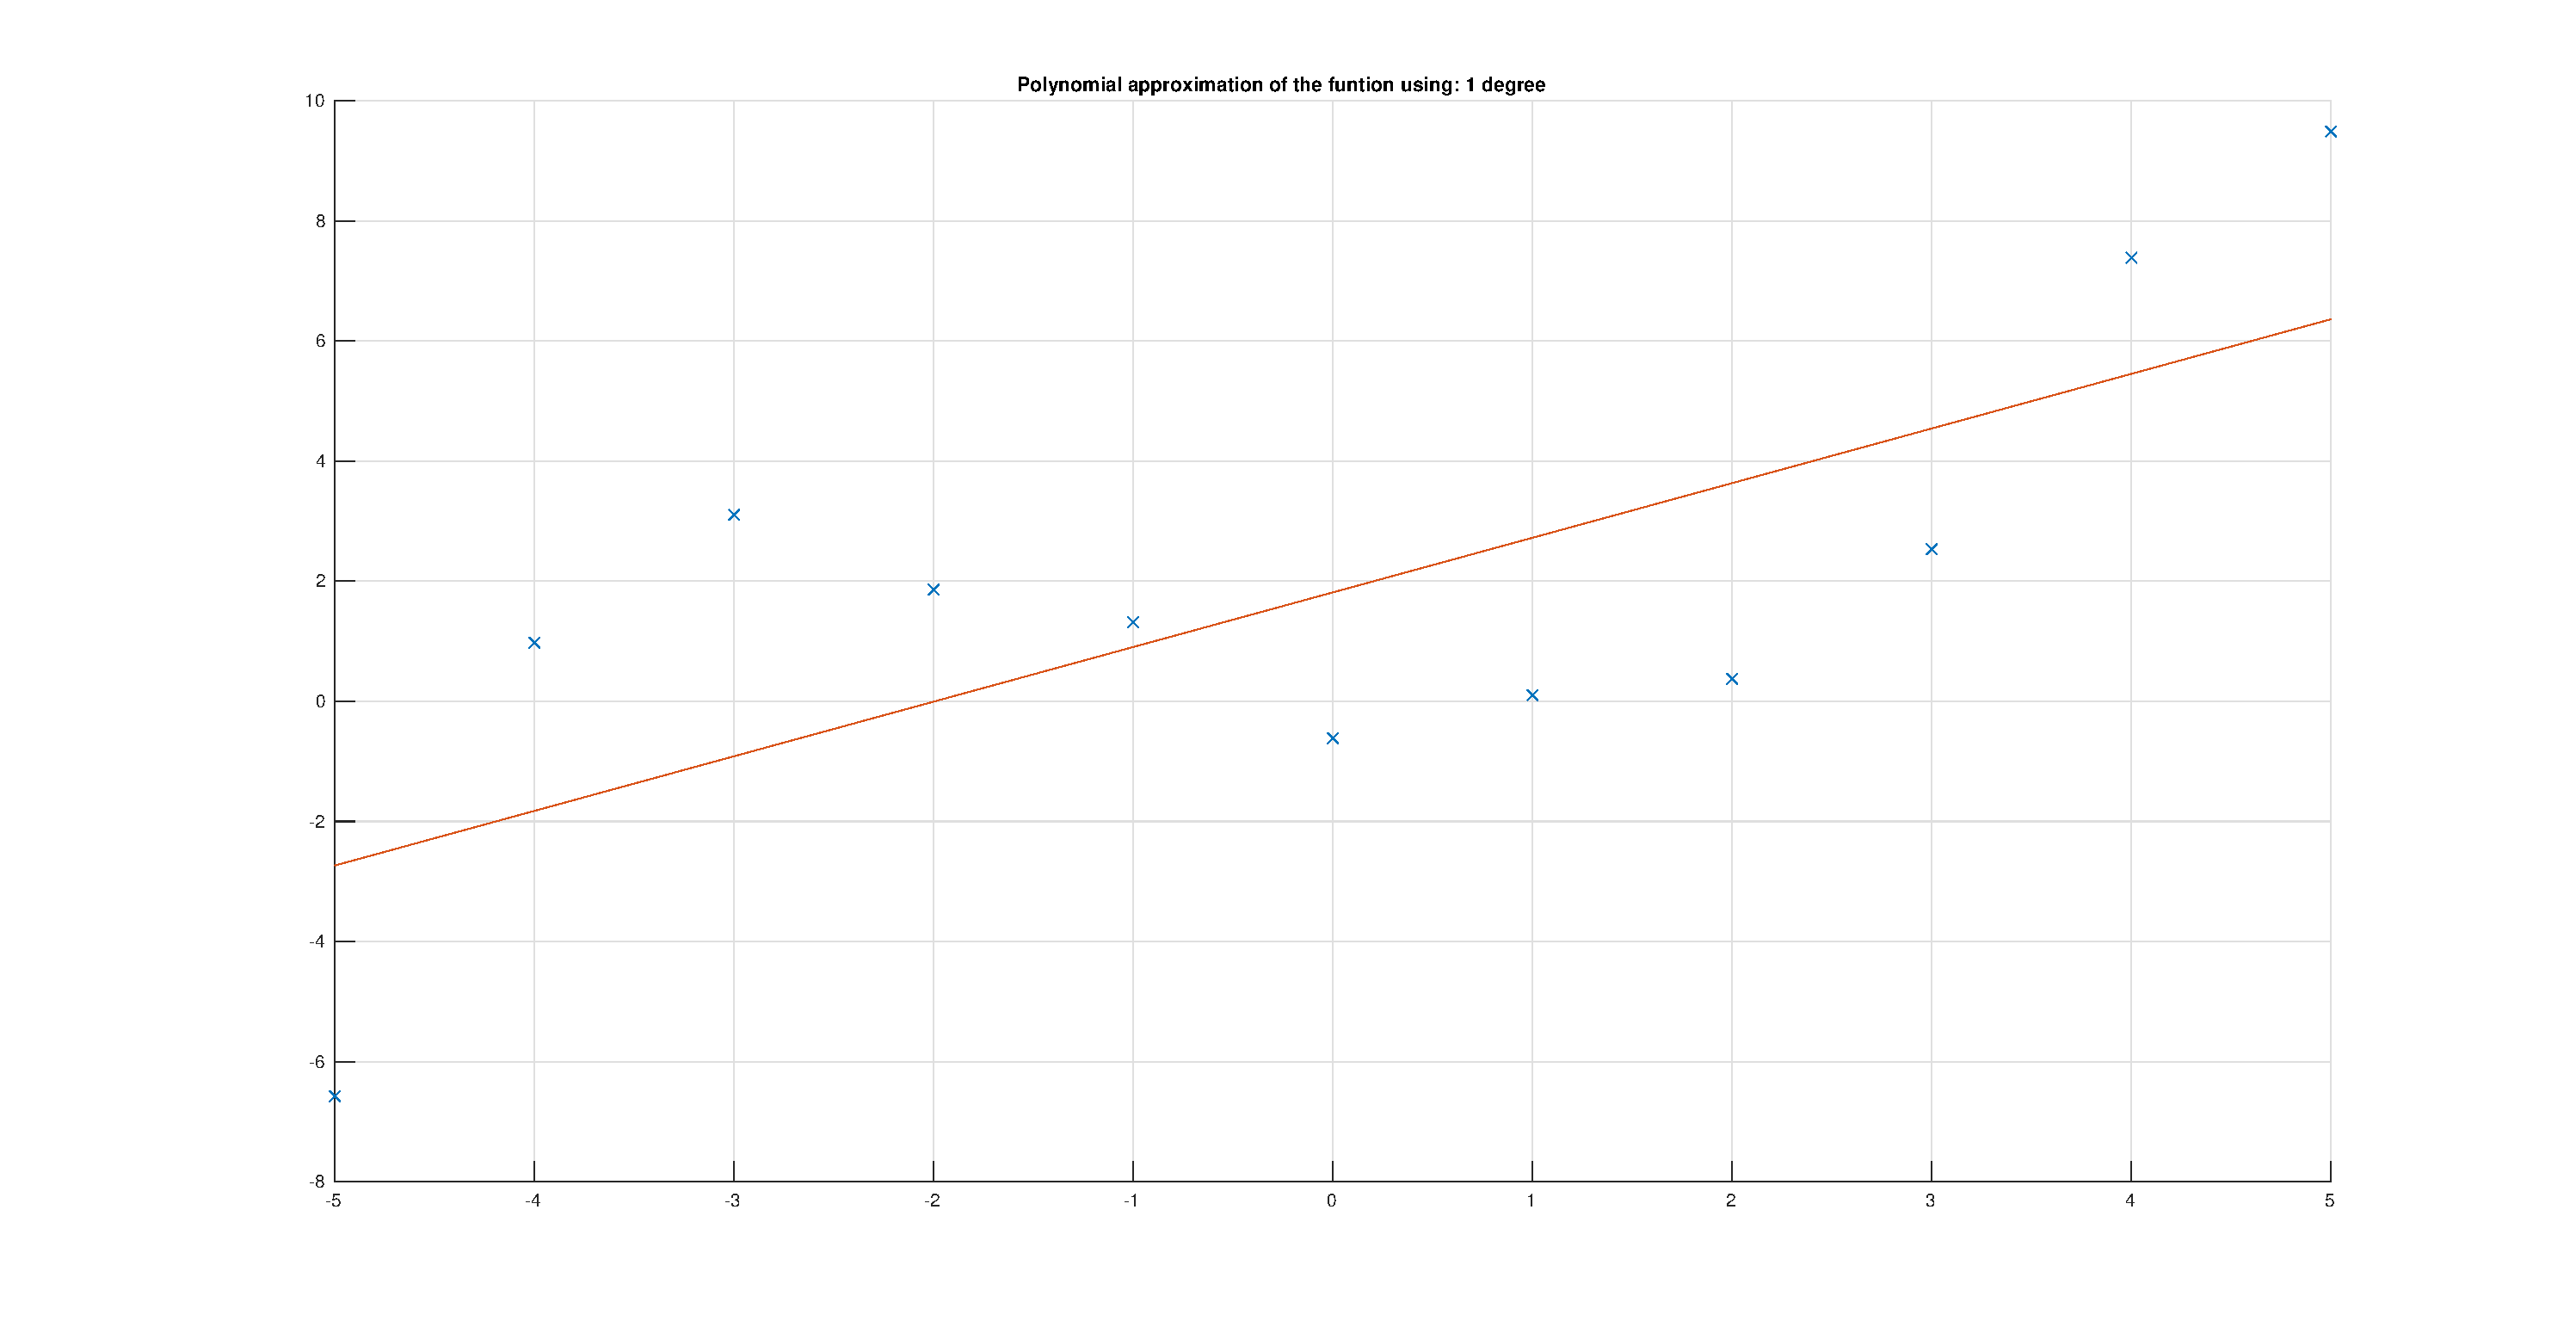
\includepdf[pages=-]{11-eps-converted-to.pdf}
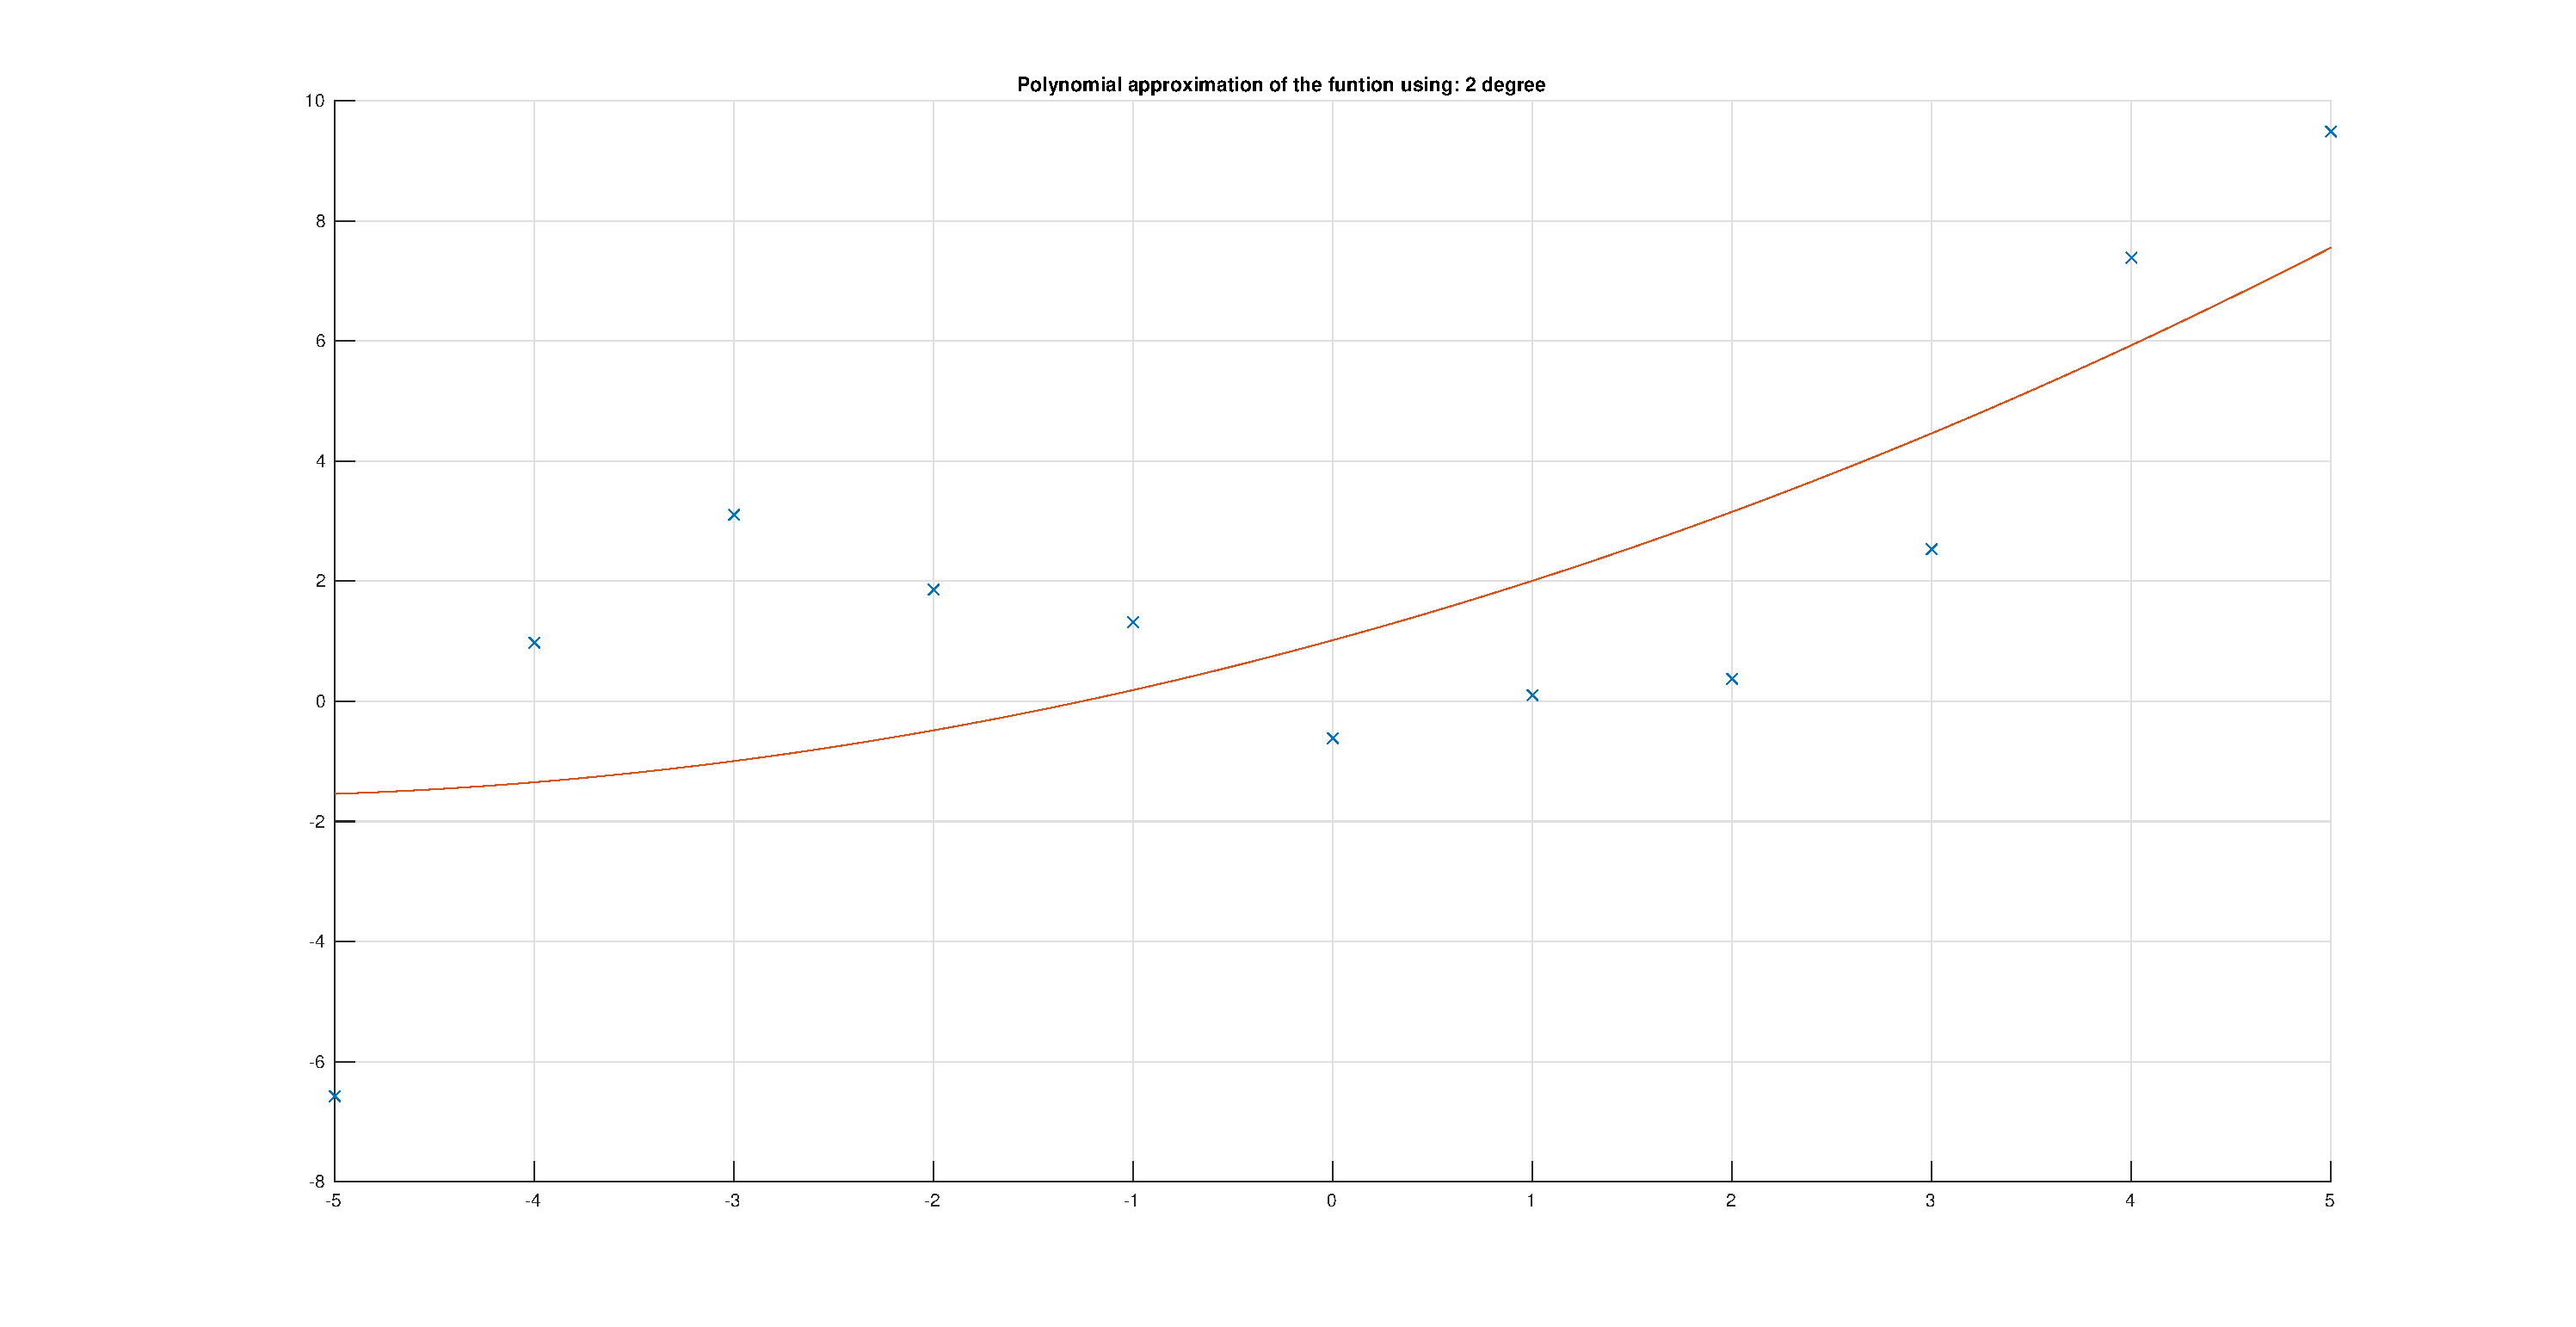
\includepdf[pages=-]{12-eps-converted-to.pdf}
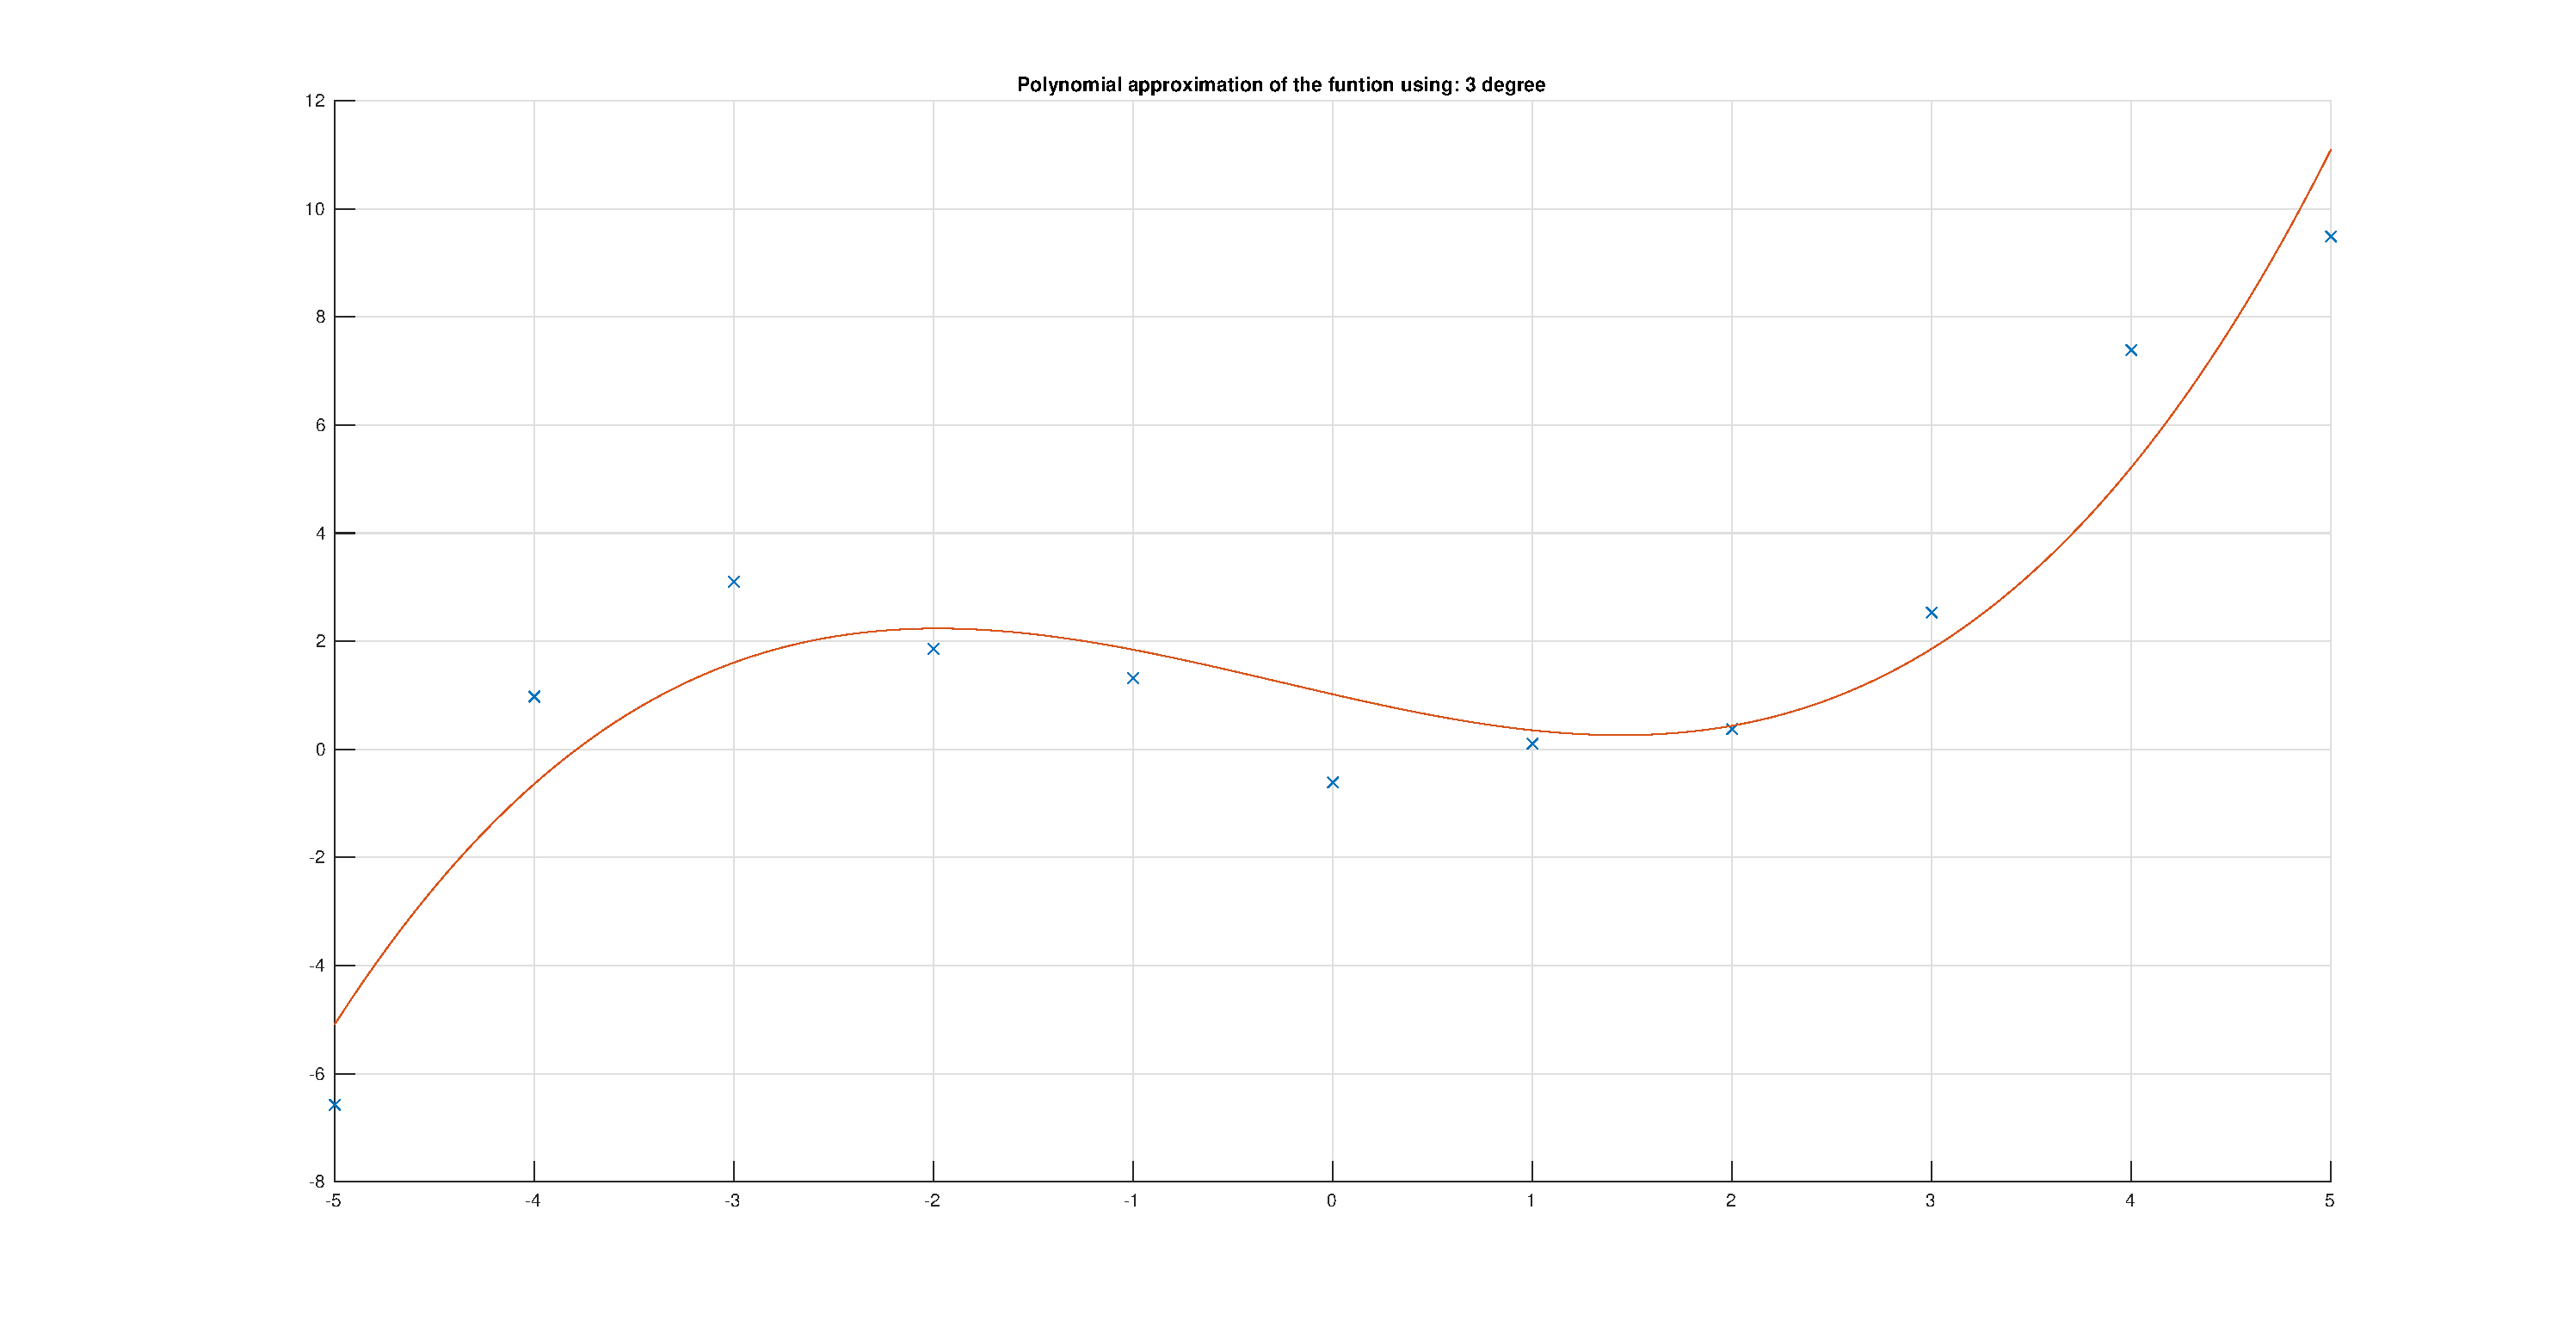
\includepdf[pages=-]{13-eps-converted-to.pdf}
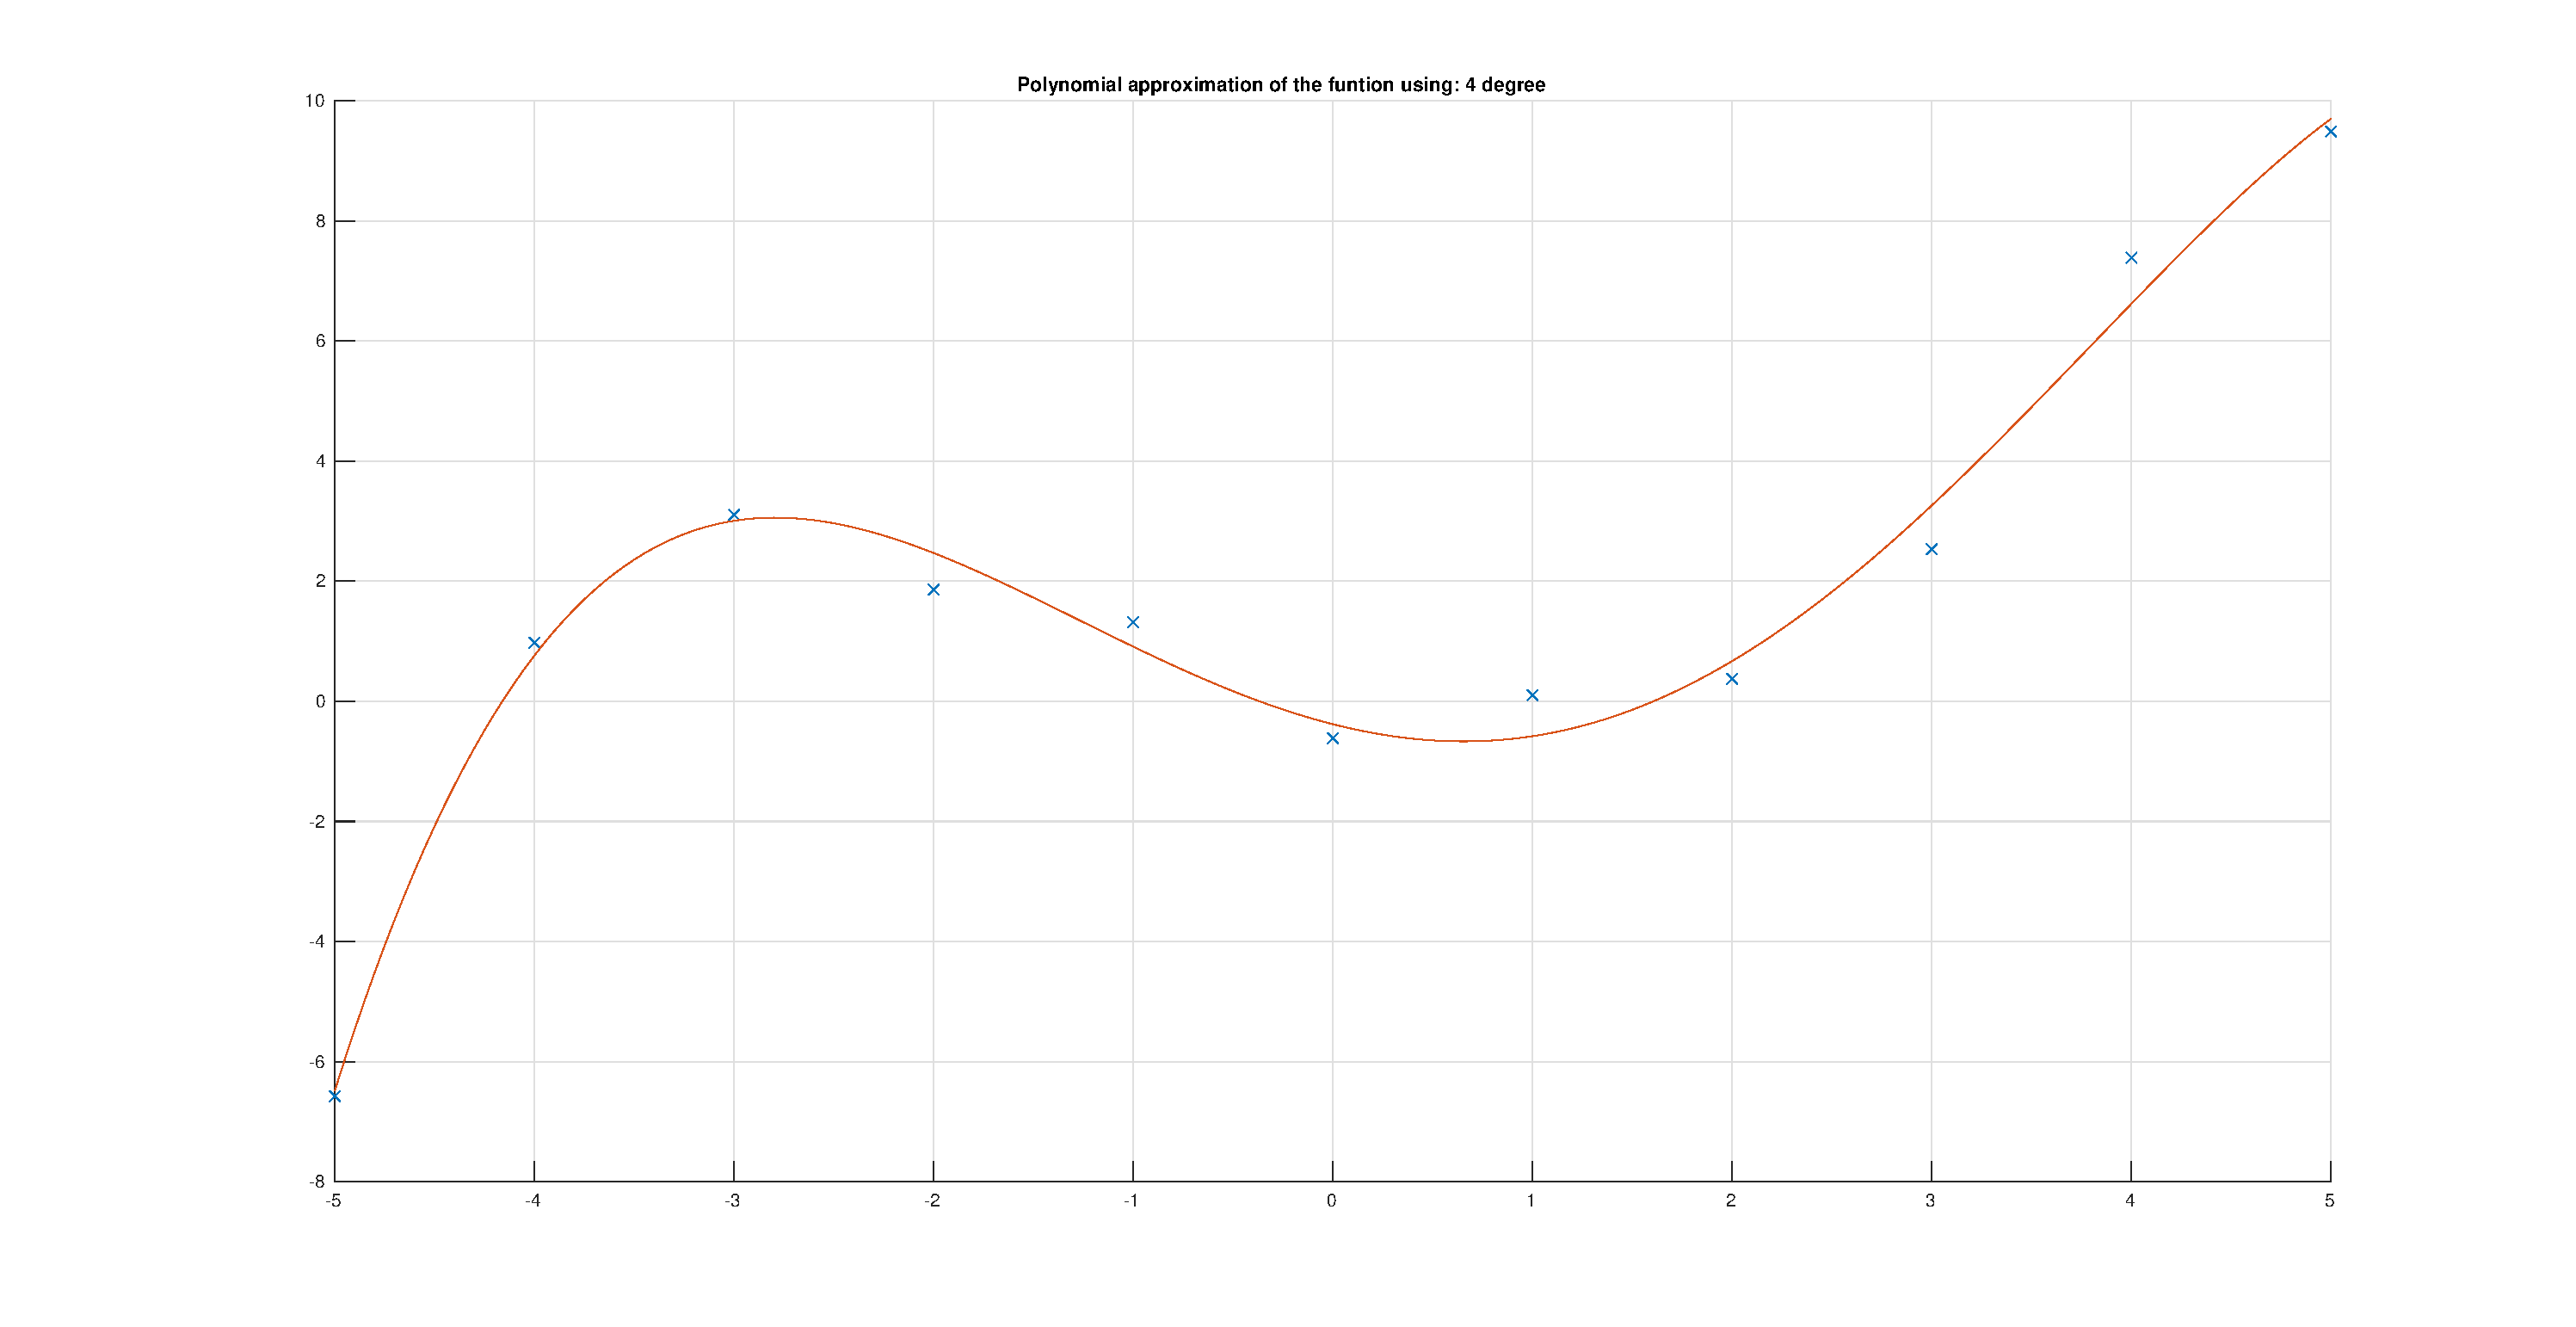
\includepdf[pages=-]{14-eps-converted-to.pdf}
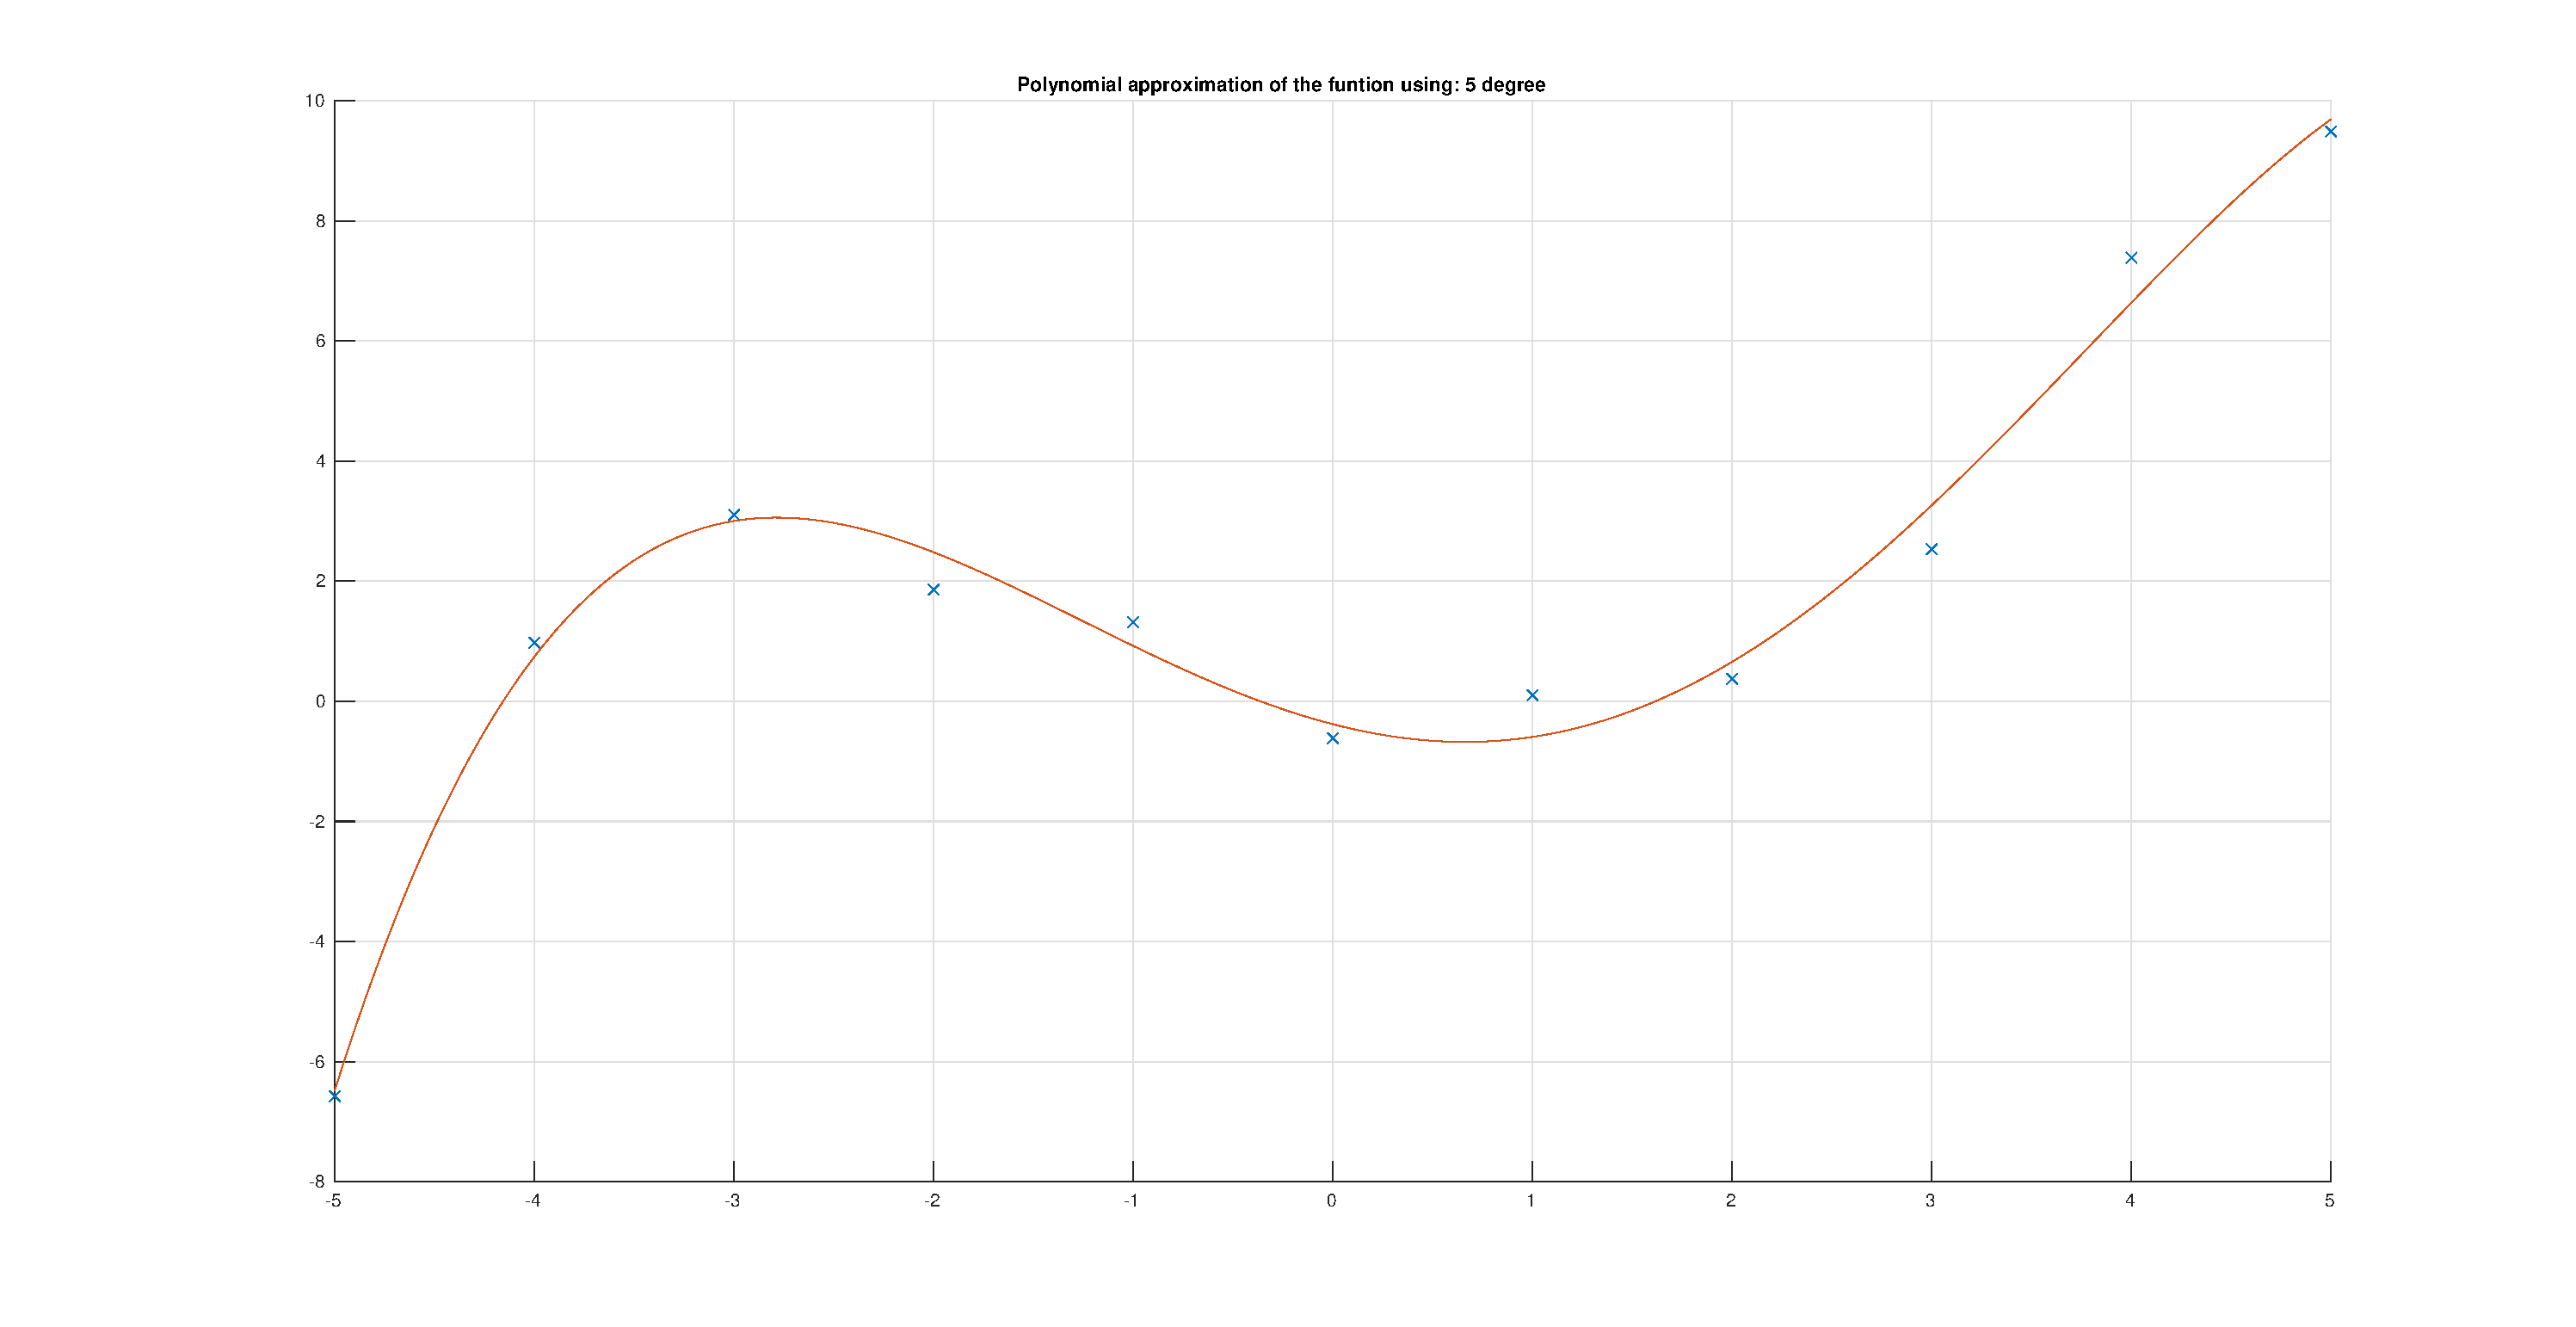
\includepdf[pages=-]{15-eps-converted-to.pdf}
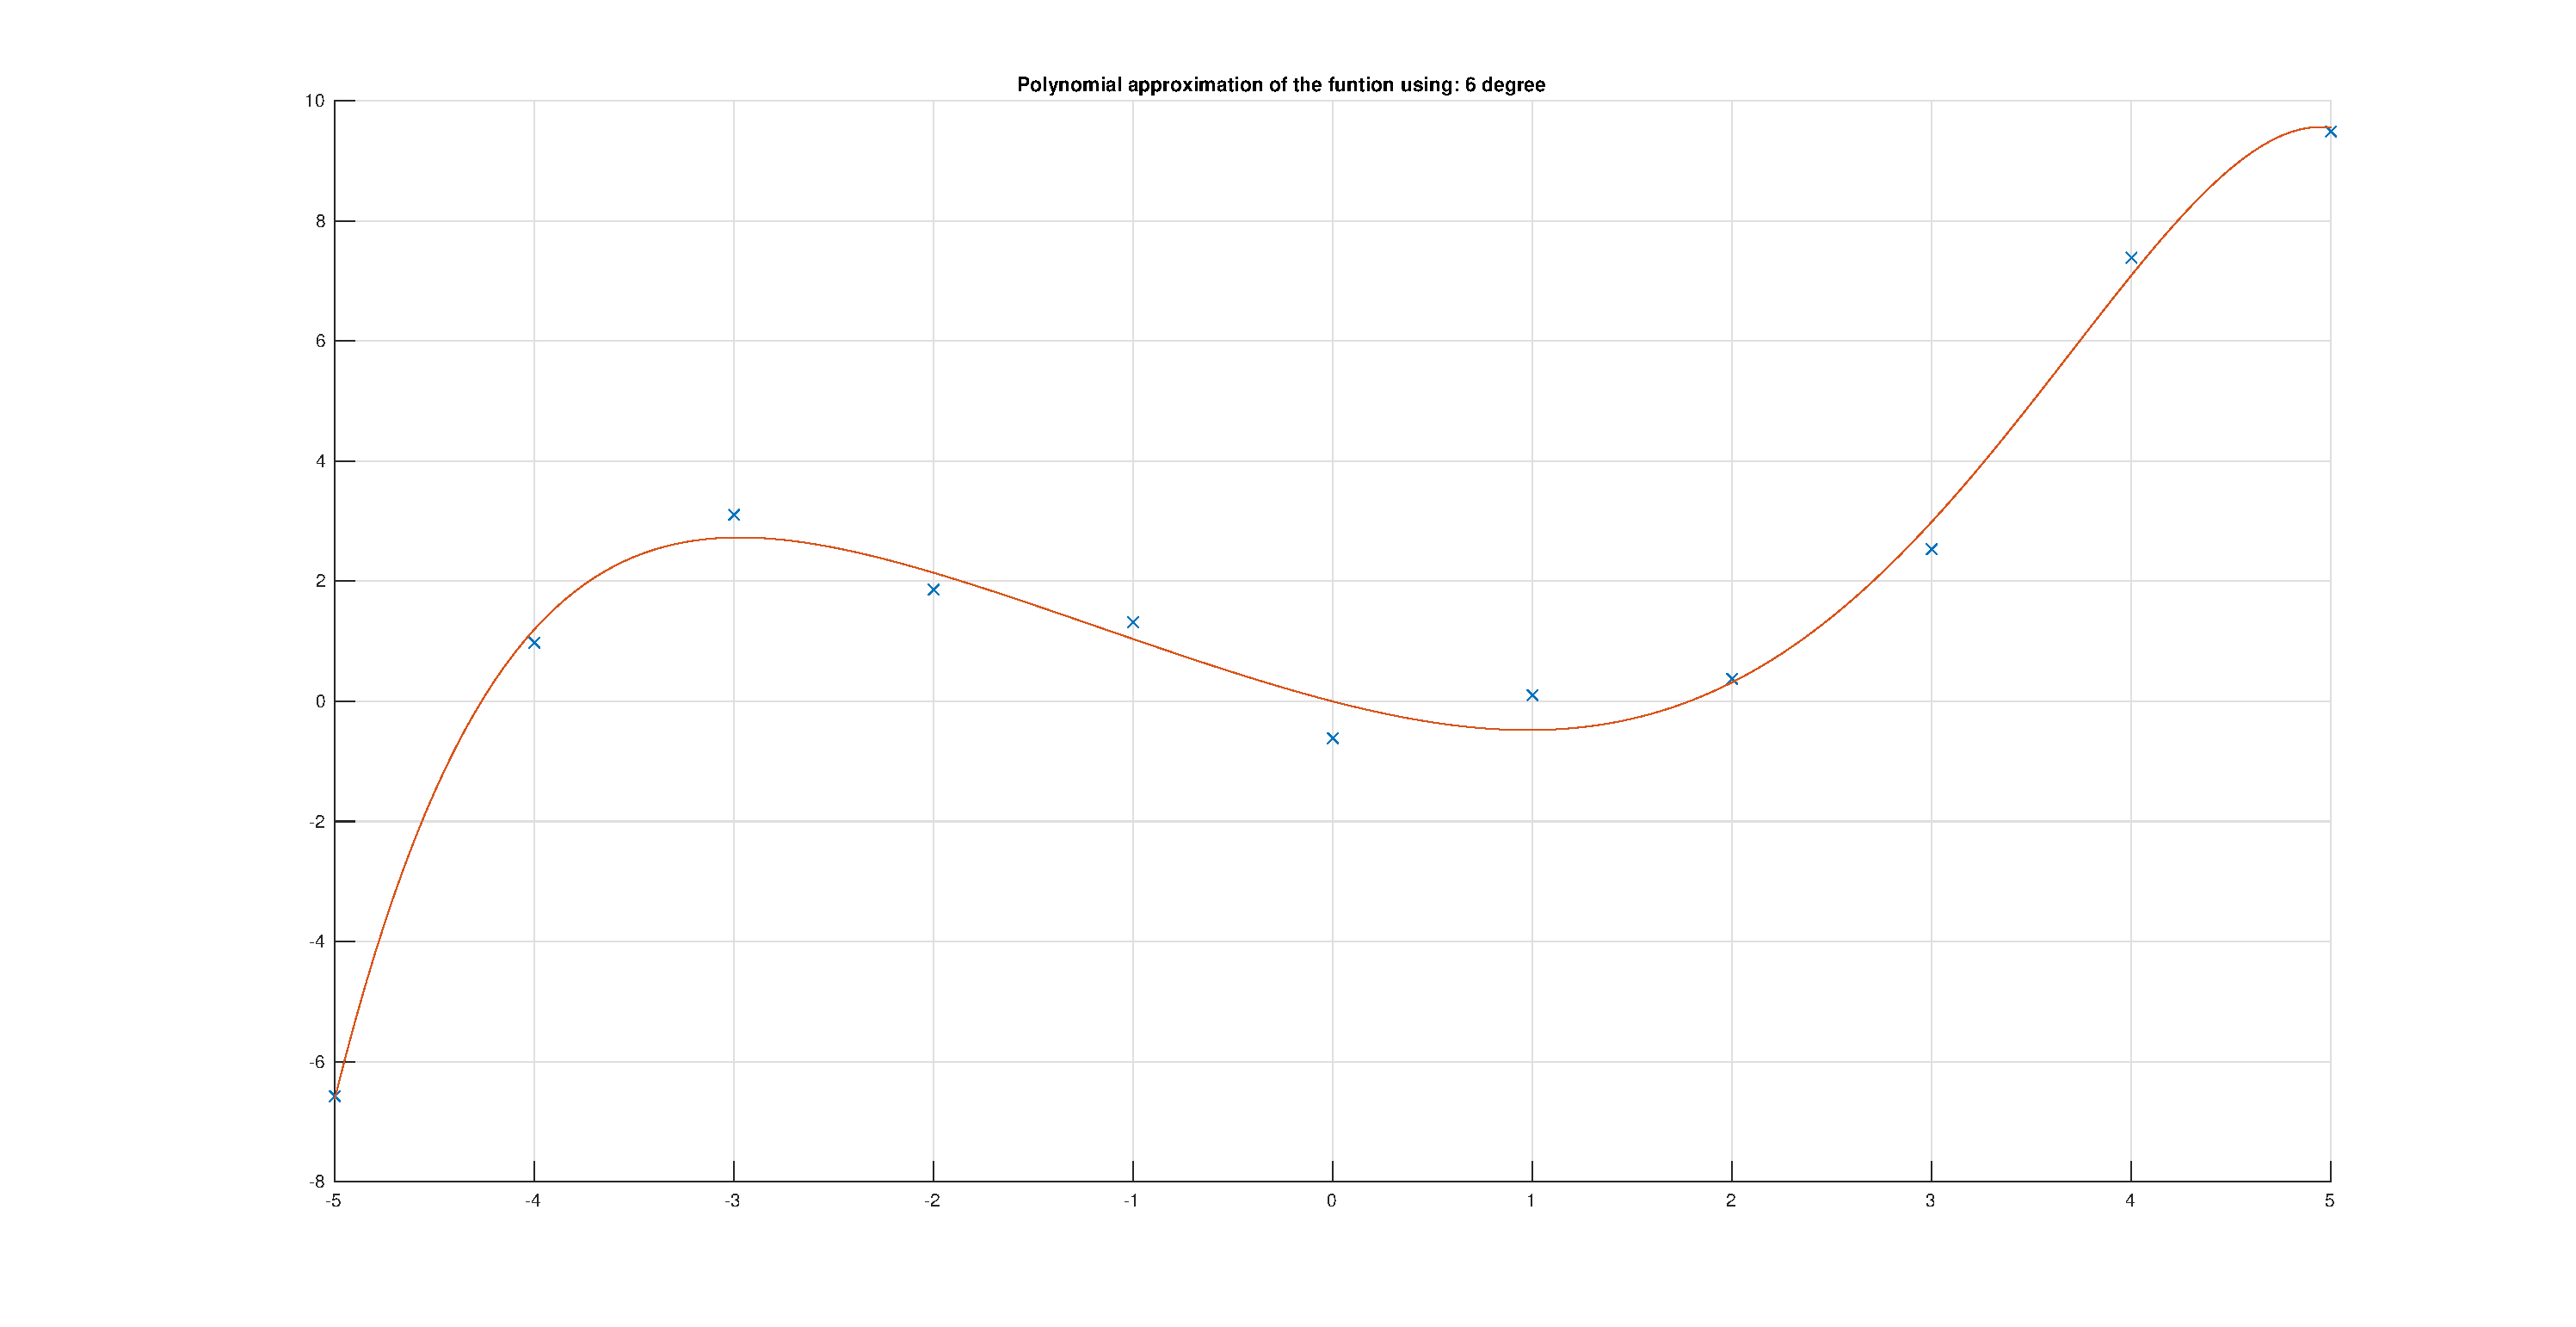
\includepdf[pages=-]{16-eps-converted-to.pdf}
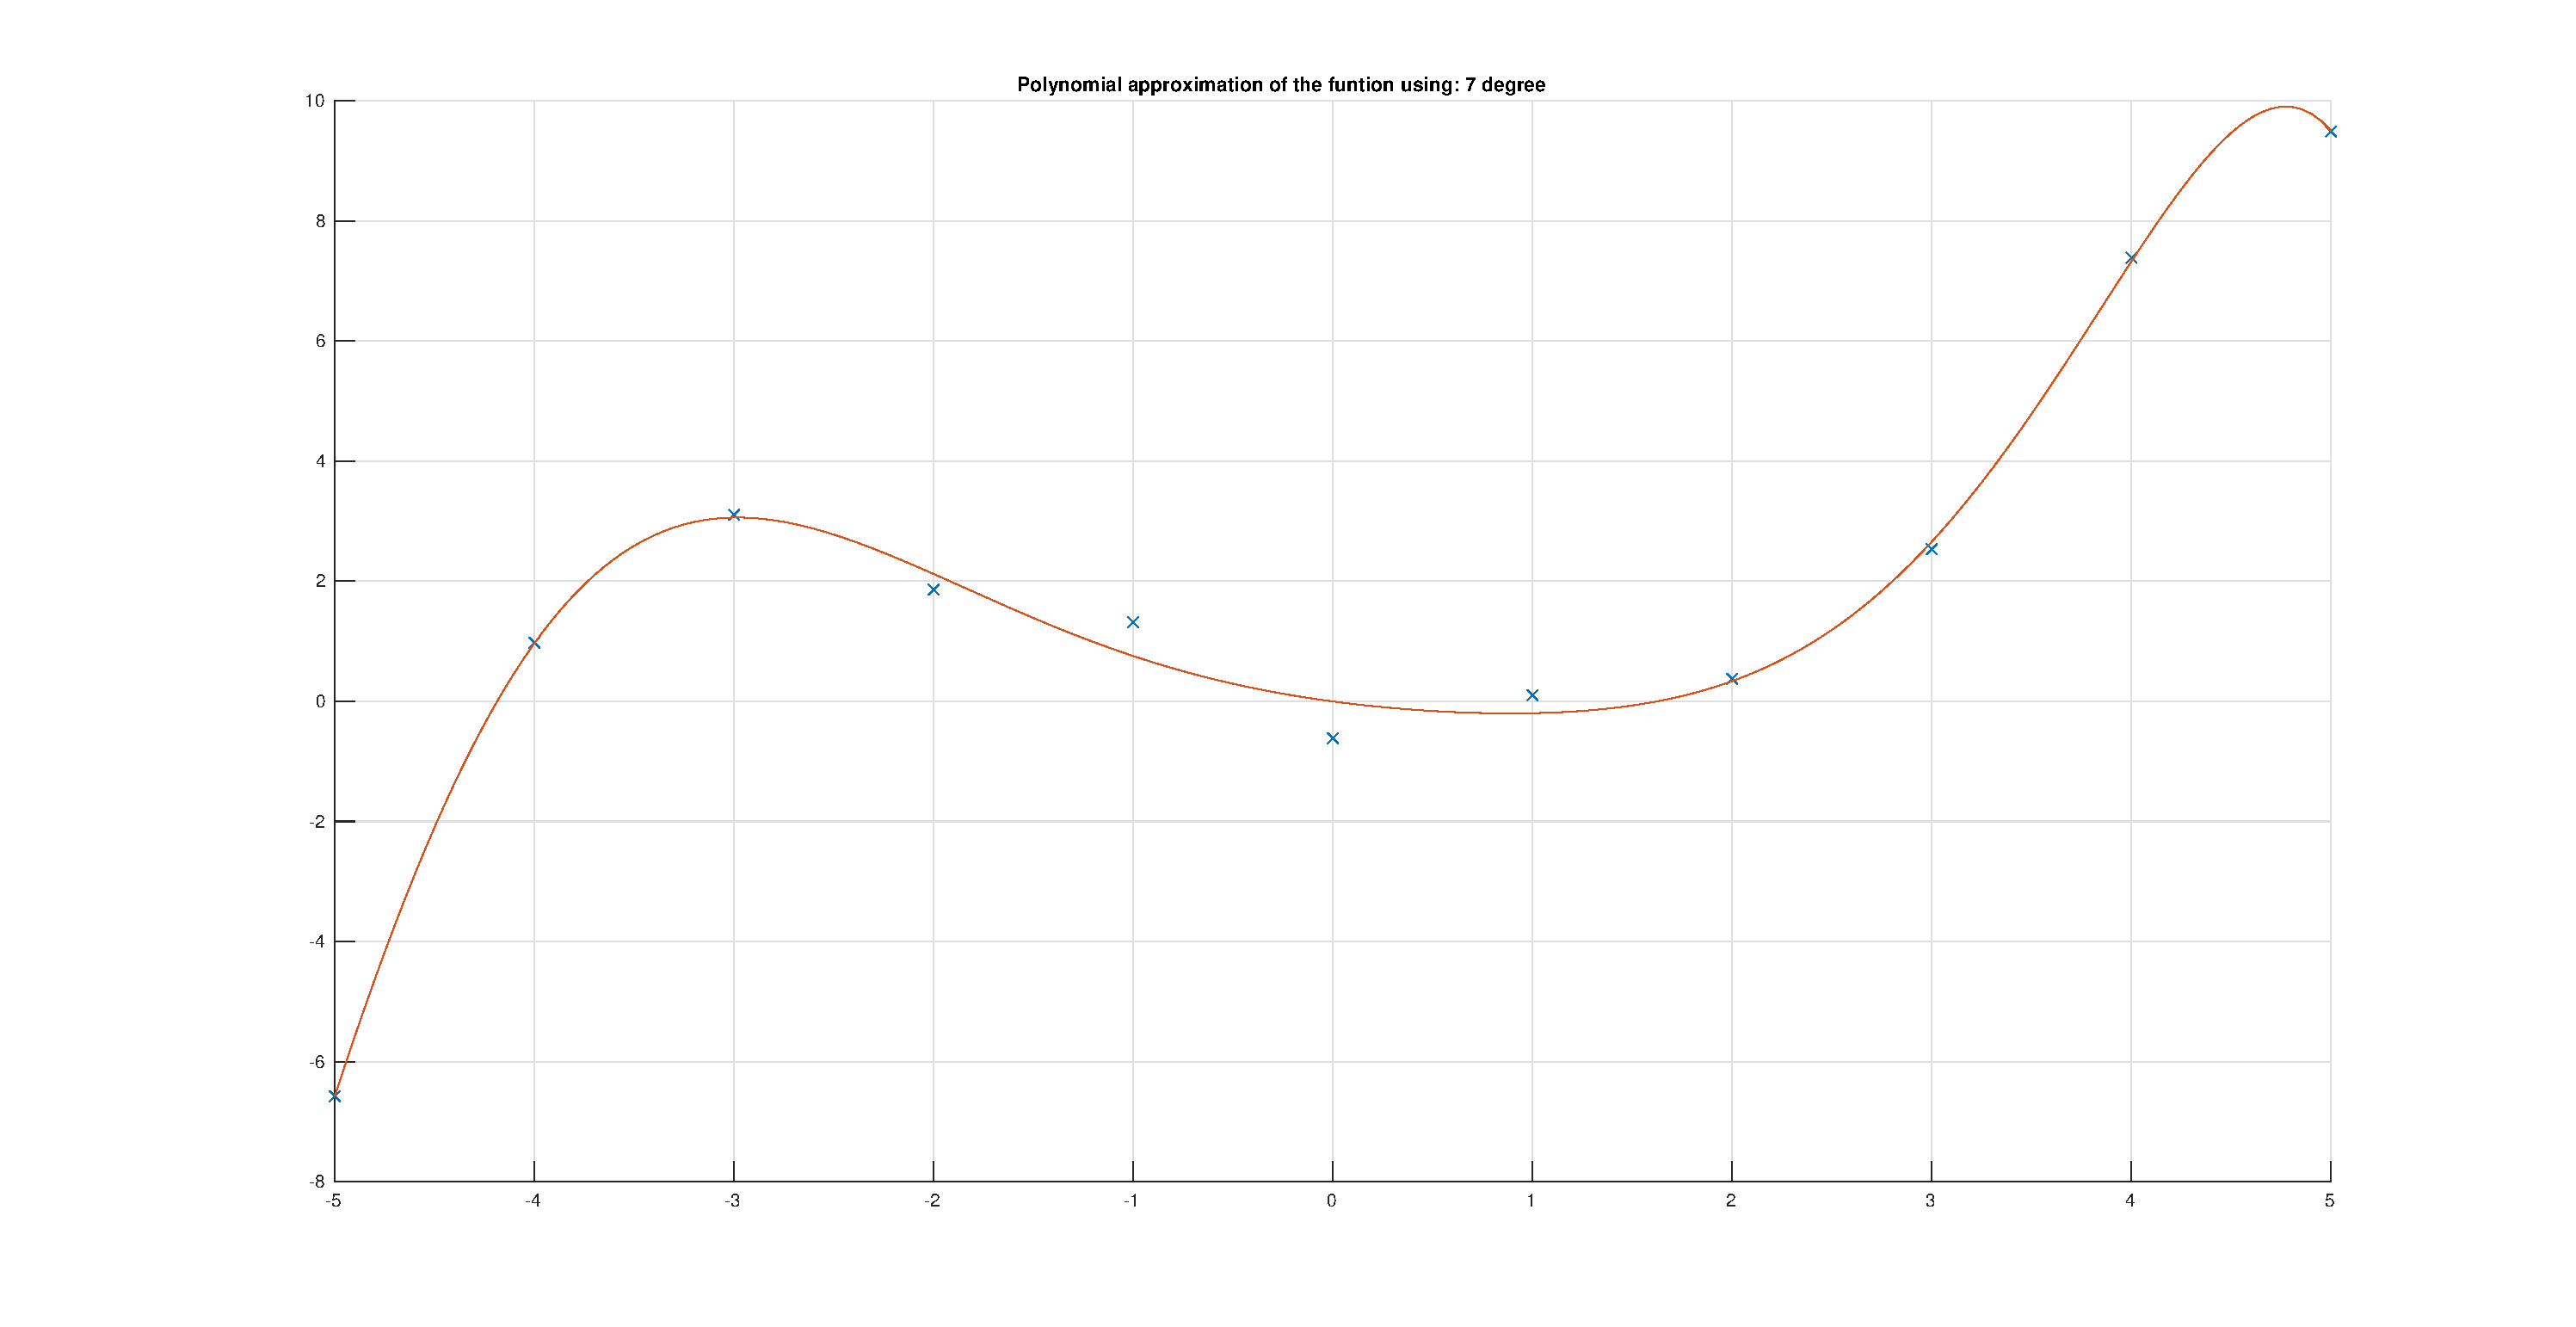
\includepdf[pages=-]{17-eps-converted-to.pdf}
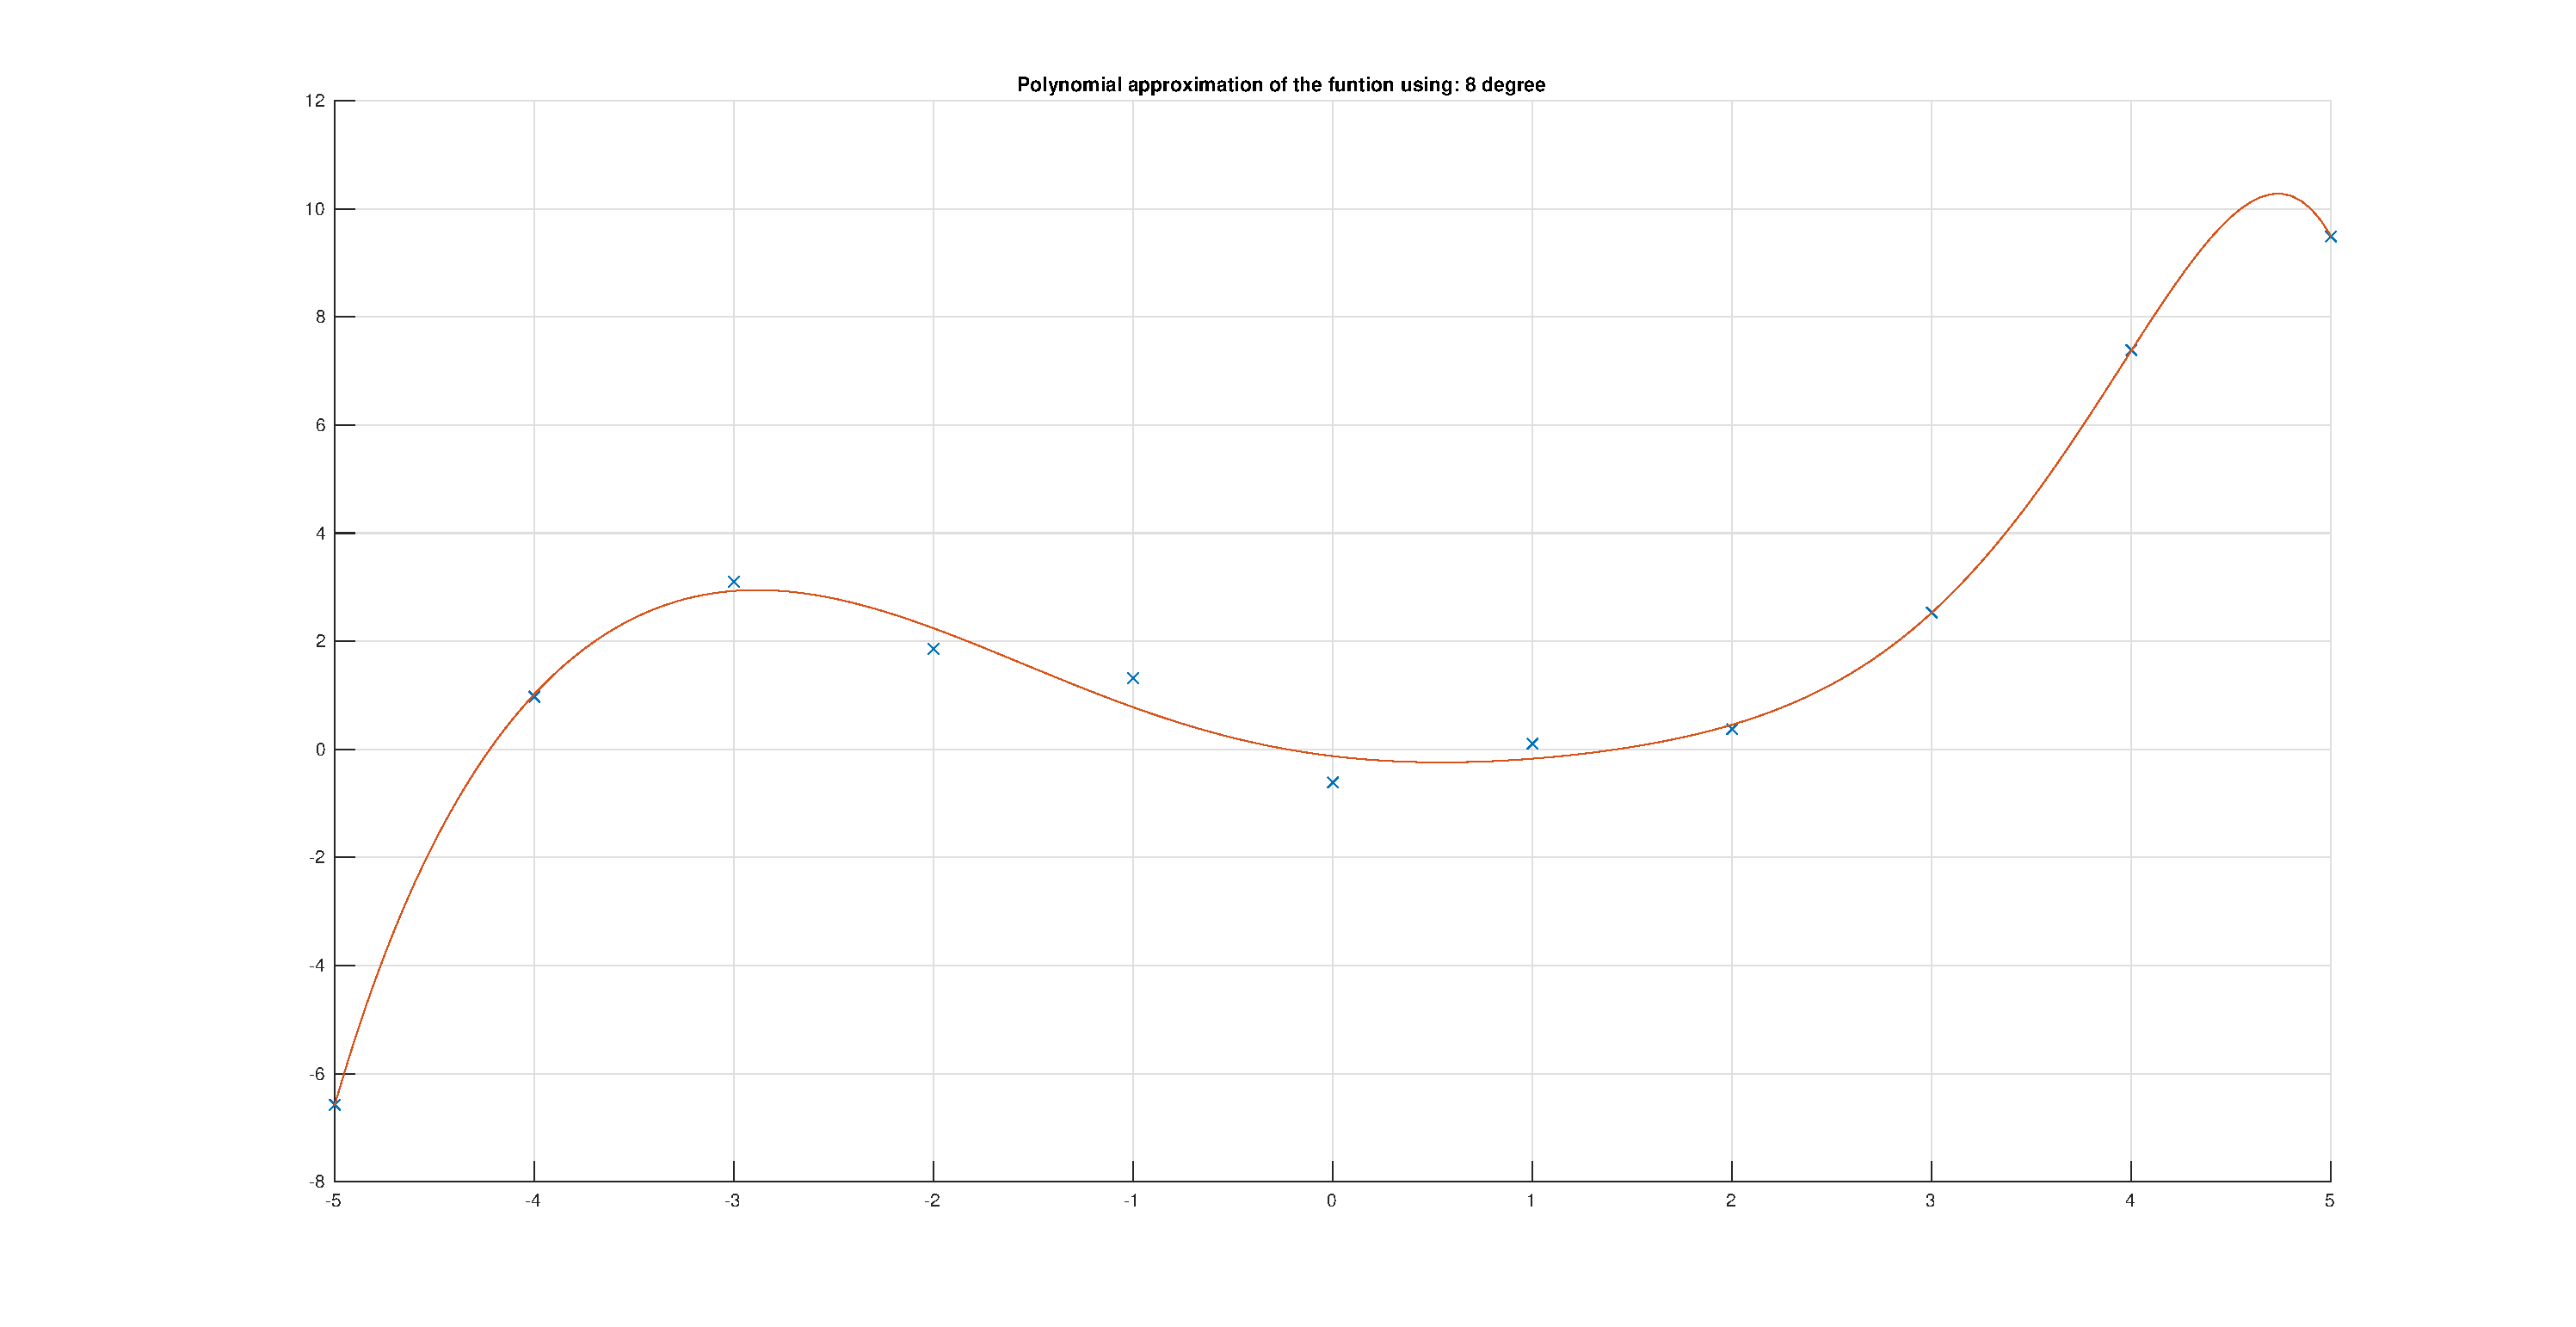
\includepdf[pages=-]{18-eps-converted-to.pdf}
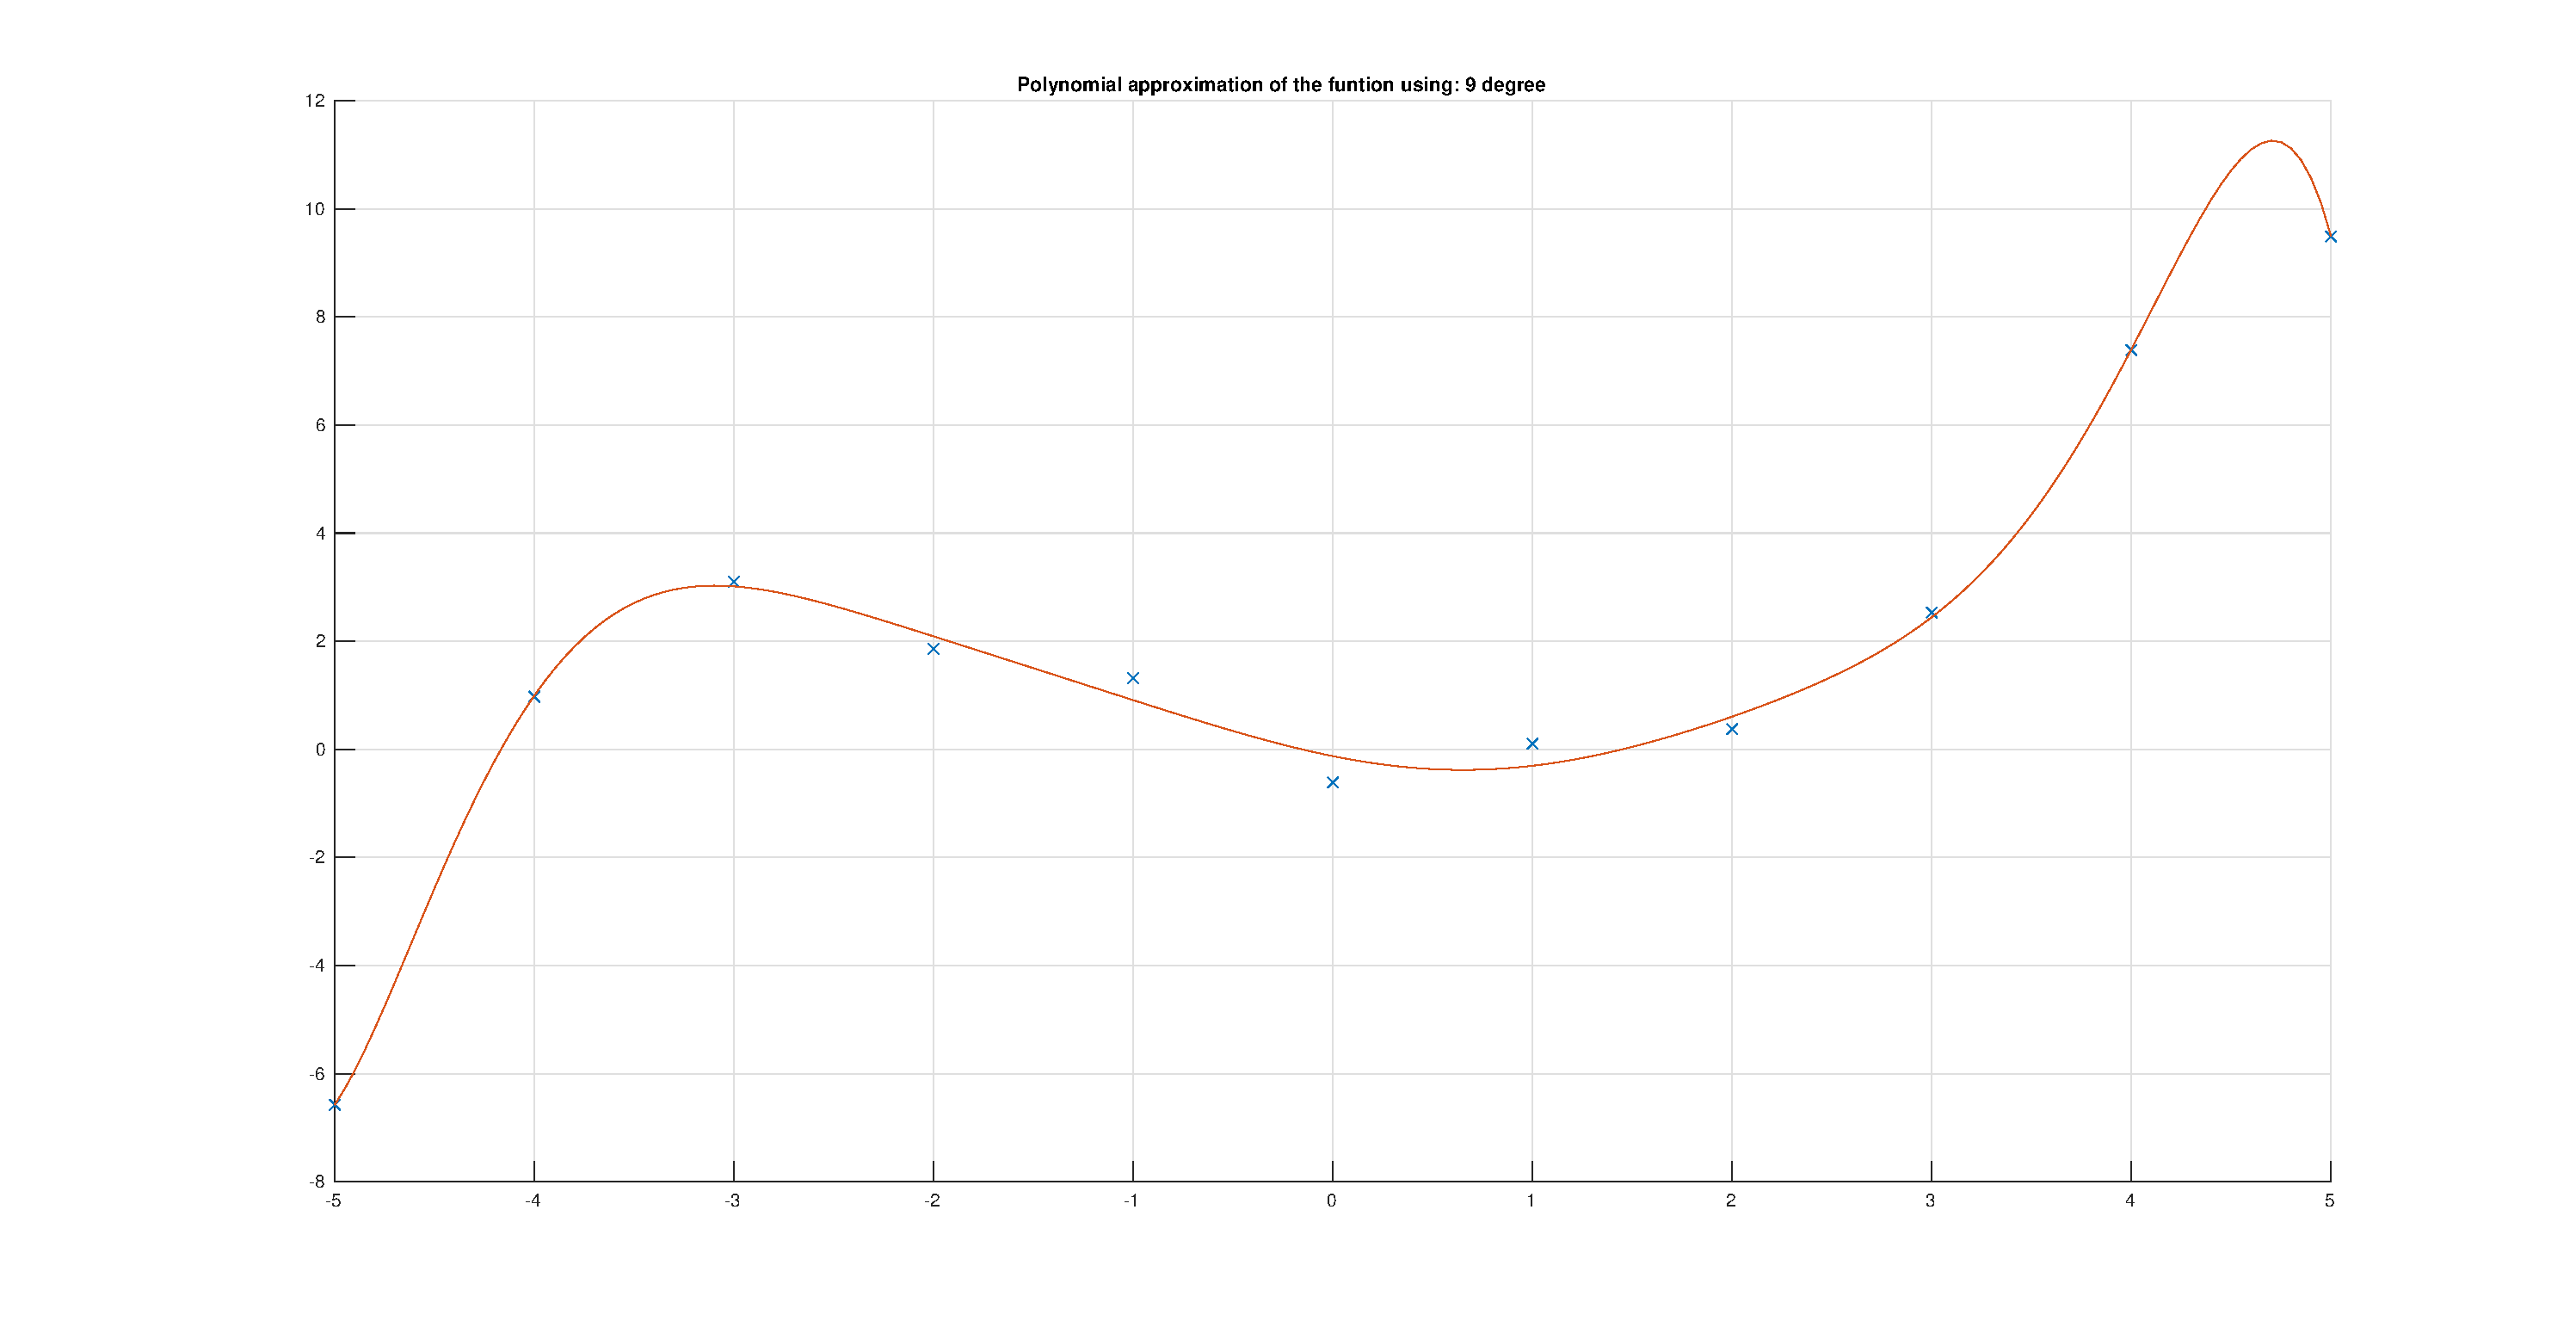
\includepdf[pages=-]{19-eps-converted-to.pdf}
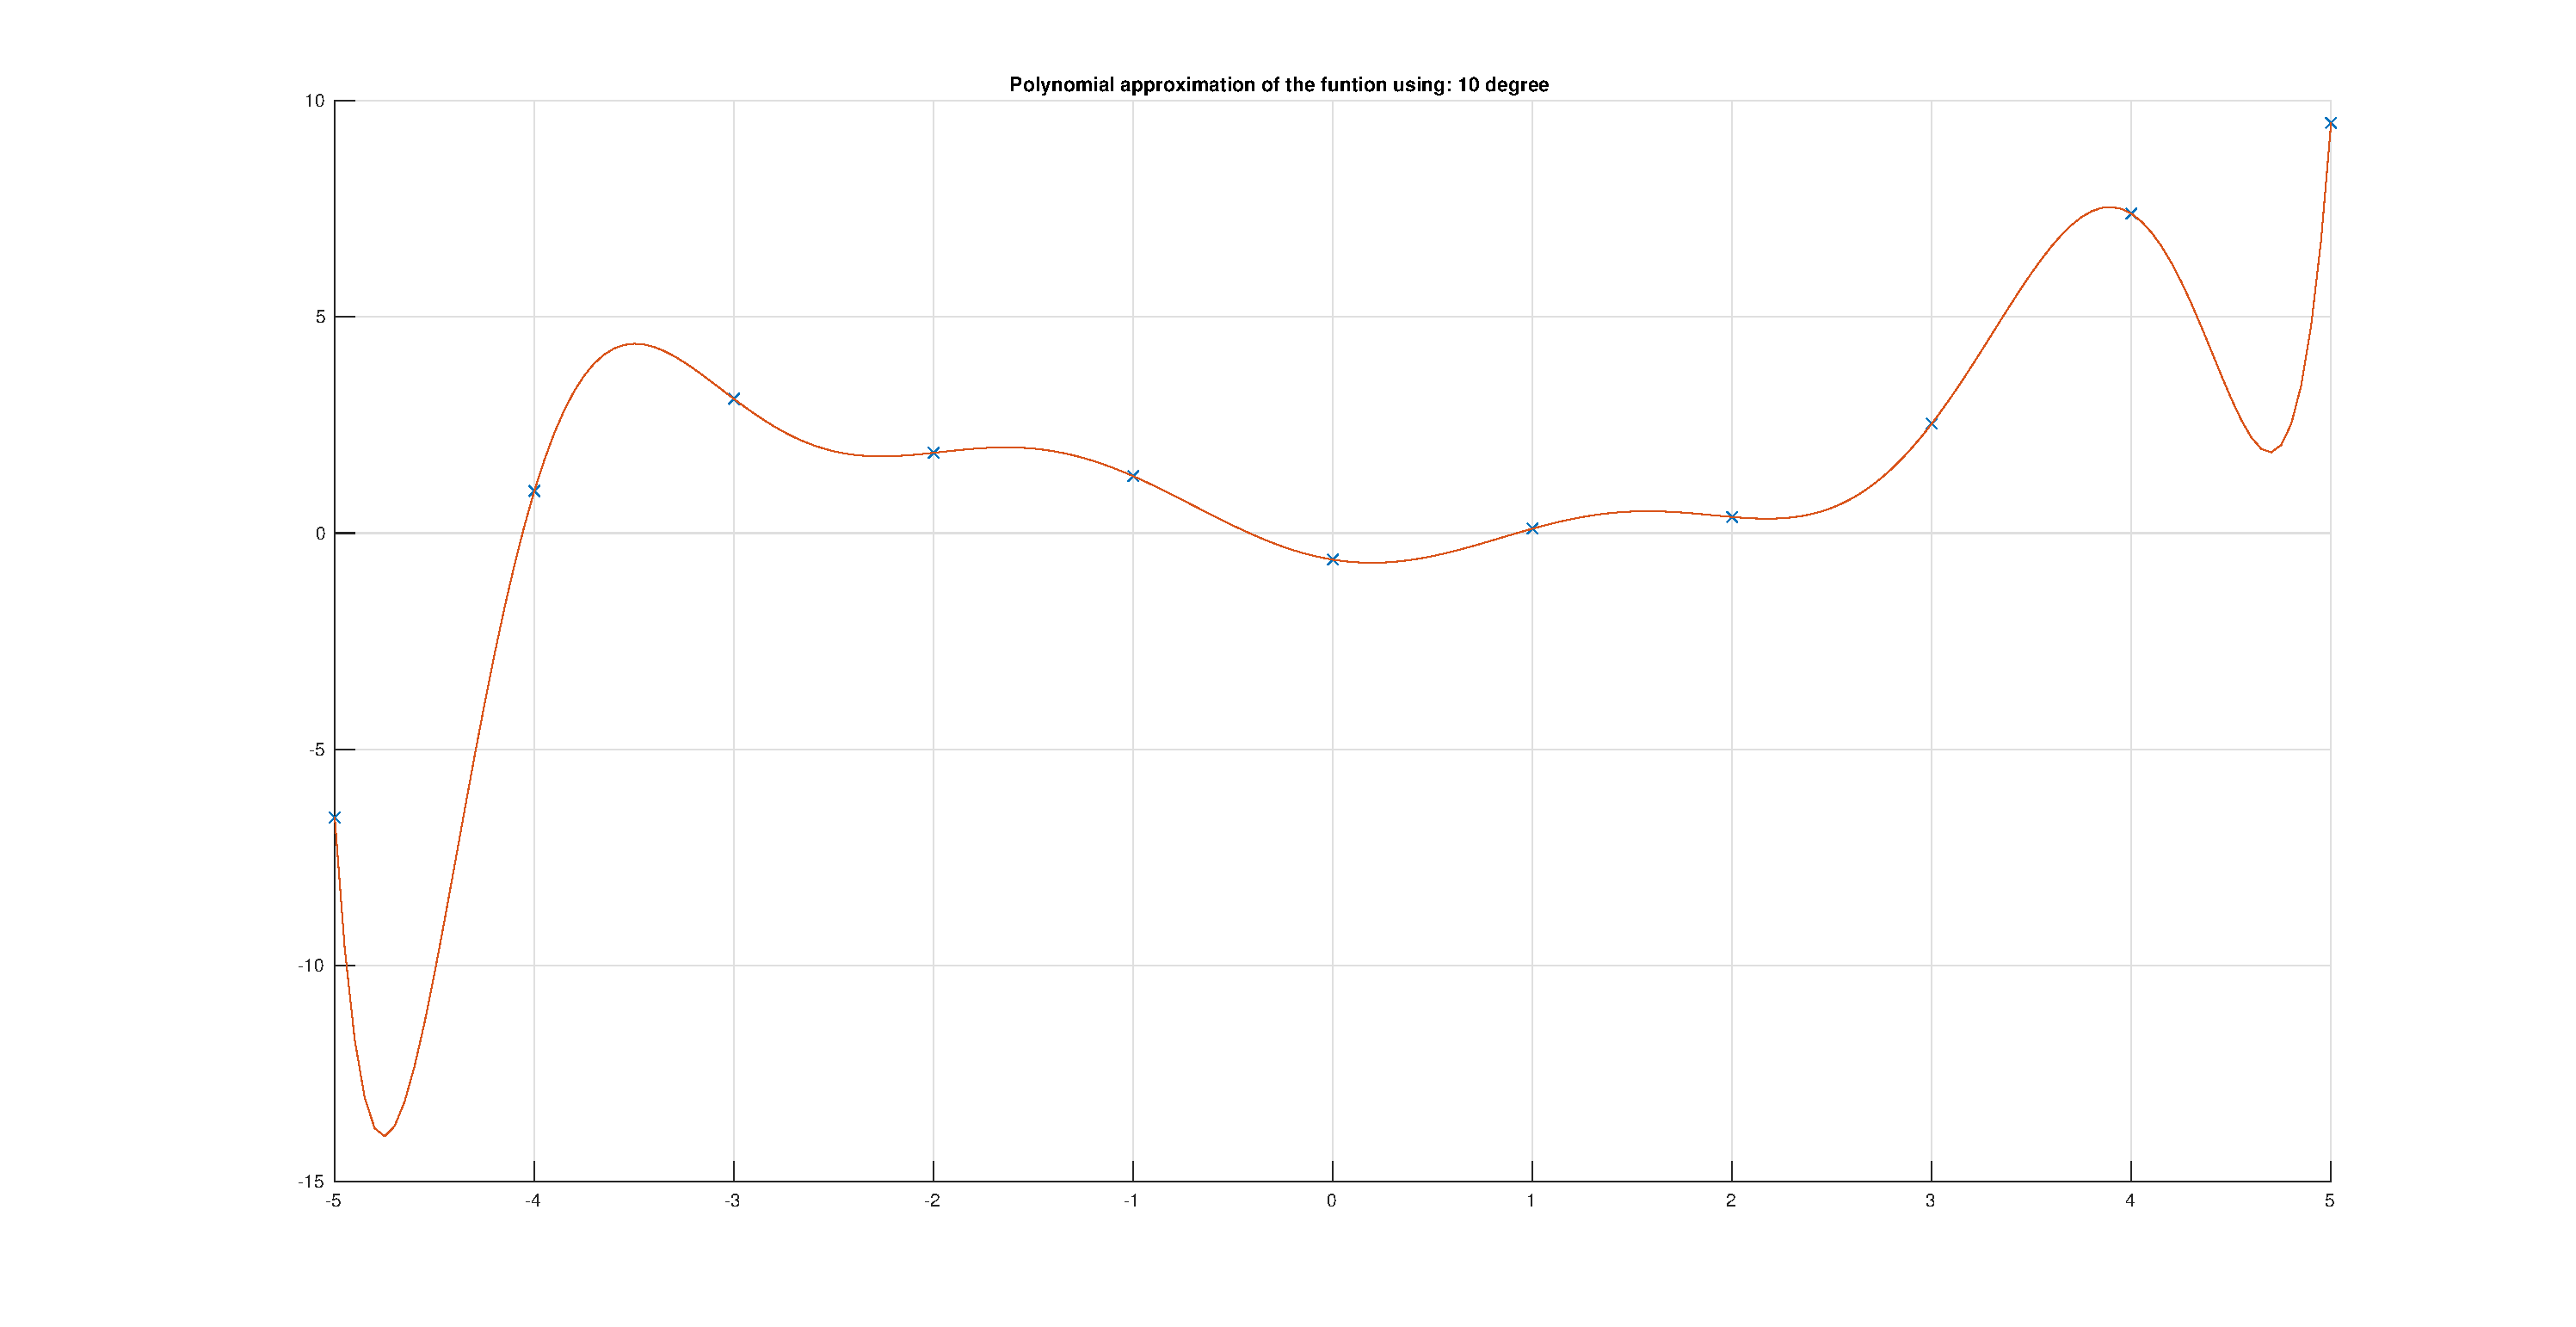
\includepdf[pages=-]{110-eps-converted-to.pdf}
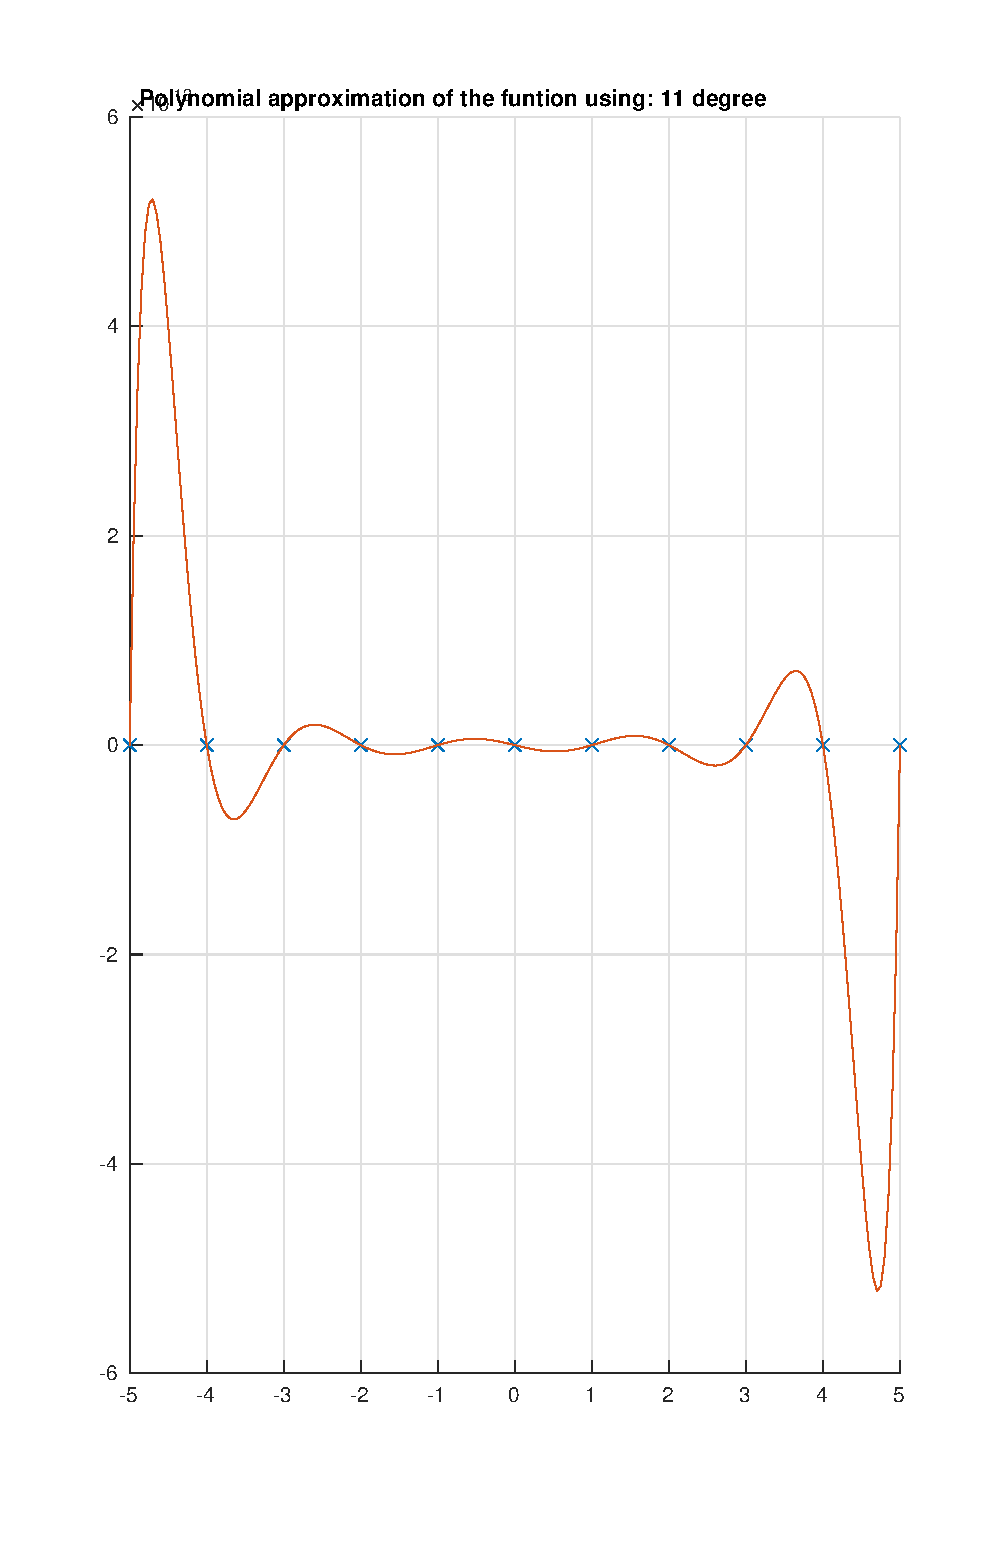
\includepdf[pages=-]{111-eps-converted-to.pdf}

\begin{center}
  \begin{tabular}{| c | c | c |}
\hline

Degree & Error & Condition number of Gram's Matrix \\
\hline
0& 13.2040& 1\\
\hline
1& 9.1281& 10\\
\hline
2& 8.8257&   408.7796\\
\hline
3& 4.2365& 8.5584e+03\\
\hline
4& 1.5418&  3.1798e+05\\
\hline
5& 1.5413& 7.4675e+06\\
\hline
6& 1.1689& 2.8316e+08\\
\hline
7& 0.9345& 7.6462e+09\\
\hline
8& 0.8883& 3.3055e+11\\
\hline
9& 0.8334& 1.5167e+13\\
\hline
10& 6.3645e-13& 9.2930e+14\\
\hline
11 & 2.2390 & 8.7763e+17 \\
\hline
  \end{tabular}
\end{center}

